\documentclass{report}
\usepackage[utf8]{inputenc}
\RequirePackage[numbers]{natbib}
\usepackage[intoc,french]{nomencl}
\makenomenclature
\renewcommand{\nomname}{Notations}
\usepackage{etoolbox}
\usepackage{subcaption}

\usepackage{chngcntr}\AtBeginDocument{\counterwithin{figure}{section}}

%%%%%%%%%%%%%%%%%%%%%%%%%%%%%%%%%%%%%%%%%%%%%%%%%%%%%%%%%%%
%%%%%  		 latin abbreviations                  %%%%%
%%%%%%%%%%%%%%%%%%%%%%%%%%%%%%%%%%%%%%%%%%%%%%%%%%%%%%%%%%%
\newcommand{\ie}{{\em i.e.,~}}
\newcommand{\eg}{{\em e.g.,~}}
\newcommand{\lcf}{{\em cf.~}}



%%%%%%%%%%%%%%%%%%%%%%%%%%%%%%%%%%%%%%%%%%%%%%%%%%%%%%%%%%%
%%%%%  		 Style math                         %%%%%
%%%%%%%%%%%%%%%%%%%%%%%%%%%%%%%%%%%%%%%%%%%%%%%%%%%%%%%%%%%

\newcommand{\nset}{\mathbb{N}}
\newcommand{\zset}{\mathbb{Z}}
\newcommand{\rset}{\mathbb{R}}
\newcommand{\cset}{\mathbb{C}}
\newcommand{\qset}{\mathbb{Q}}
\usepackage{xifthen}
\newcommand{\EE}[1][]{%
  \ifthenelse{\isempty{#1}}%
    {\mathbb{E}}% if #1 is empty
    {\mathbb{E}\left[#1\right]}% if #1 is not empty
}

\newcommand{\PP}[1][]{%
  \ifthenelse{\isempty{#1}}%
    {\mathbb{P}}% if #1 is empty
    {\mathbb{P}\left(#1\right)}% if #1 is not empty
}


\def\1{\mathbf 1}
\newcommand{\mb}{\mathbf}
\newcommand{\ud}{\,\mathrm{d}} 
\newcommand{\given}[1][{}]{\;\middle\vert\;{#1} }
\def\indep{\perp\!\!\!\perp}


%%%%%%%%%%%%%%%%%%%%%%%%%%%%%%%%%%%%%%%%%%%%%%%%%%%%%%%%%%%
%%%%%        defintion symbols                        %%%%%
%%%%%%%%%%%%%%%%%%%%%%%%%%%%%%%%%%%%%%%%%%%%%%%%%%%%%%%%%%%
\newcommand{\deq}{\stackrel{def}{=}}


%%%%%%%%%%%%%%%%%%%%%%%%%%%%%%%%%%%%%%%%%%%%%%%%%%%%%%%%%%%
%%%%%        maths symbols                    	     %%%%%
%%%%%%%%%%%%%%%%%%%%%%%%%%%%%%%%%%%%%%%%%%%%%%%%%%%%%%%%%%%
\usepackage{amsopn}
\DeclareMathOperator{\sign}{sign}
\DeclareMathOperator{\Card}{Card}
\DeclareMathOperator{\rg}{rg}
\DeclareMathOperator{\tr}{tr}
\DeclareMathOperator{\corr}{corr}
\DeclareMathOperator{\var}{var}
\DeclareMathOperator{\vect}{vect}

\DeclareMathOperator{\cov}{cov}
\DeclareMathOperator{\pred}{pred}
\DeclareMathOperator{\Id}{Id}

\newcommand{\argmin}{\mathop{\mathrm{arg\,min}}}
\newcommand{\argmax}{\mathop{\mathrm{arg\,max}}}
\def\rang{\mathop{\rm rang}\nolimits}
\def\Ker{\mathop{\rm Ker}\nolimits}
\def\Im{\mathop{\rm Im}\nolimits}
\def\Vect{\mathop{\rm Vect}\nolimits}



\def\dim{\mathop{\rm dim}\nolimits}
\def\Var{\mathop{\rm Var}\nolimits}
\def\Cov{\mathop{\rm Cov}\nolimits}

\def\dom{\mathop{\rm dom}\nolimits}
\def\supp{\mathop{\rm supp}\nolimits}
\def\relint{\mathop{\rm relint}\nolimits}




\def\bfr{\mathbf{r}}
\def\bfx{\mathbf{x}}
\def\bfy{\mathbf{y}}
\def\bftheta{\bm{\theta}}
\def\bfepsilon{\bm{\varepsilon}}


\def \cN{\mathcal{N}}
\def\calN{\cN}
\def\calL{\mathcal{L}}
\def\calM{\mathcal{M}}
\def\calH{\mathcal{H}}
\def \SSE{\text{SSE}}

\newcommand{\tnorm}[1]{{\left\vert\kern-0.25ex\left\vert\kern-0.25ex\left\vert #1 
    \right\vert\kern-0.25ex\right\vert\kern-0.25ex\right\vert}} % triple norm

\newcommand{\inner}[1]{{
\left\langle #1 \right\rangle}} % inner product

\newcommand{\norm}[1]{{
\left\| #1 \right\|}} % norm

\newcommand{\abs}[1]{{
\left| #1 \right|}} % norm

\newcommand{\piecewise}[1]{{
\left\lbrace \begin{array}{ll} #1 \end{array} \right. }} % for piecewise functions

\newcommand{\seg}[1]{{
\left[ #1 \right]}} % segment

\newcommand{\iseg}[1]{{
\left\llbracket #1 \right\rrbracket}} % integer segment

\newcommand{\ens}[1]{{
\left\lbrace #1 \right\rbrace }} % ensemble


%%%%%%%%%%%%%%%%%%%%%%%%%%%%%%%%%%
%%%  algo symbols %%%
\def\octave{\lstinline+Octave+}
\def\matlab{\lstinline+MATLAB+}
%%%%%%%%%%%%%%%%%%%%%%%%%%%%%%%%%%%%%%%%%%%%%%%%%%%%%%%%%%%
%%%%% 	French, accents and font coding     	      %%%%%
%%%%%%%%%%%%%%%%%%%%%%%%%%%%%%%%%%%%%%%%%%%%%%%%%%%%%%%%%%%

\usepackage[french]{babel}
\AtBeginDocument{\renewcommand\labelitemi{$\bullet$}}
\usepackage{enumitem} 
\usepackage{fancyhdr}
\usepackage[utf8]{inputenc}
\usepackage{amsmath, amssymb, amsthm}			% for theorem definitions
\usepackage[top=2cm, bottom=2cm, left=1.5cm, right=1.5cm]{geometry}


\usepackage{graphicx}			% for images and graphics
\usepackage{stmaryrd}			% for \llbracket symbols [[ ]]

%%%%%%%%%%%%%%%%%%%%%%%%%%%%%%%%%%%%%%%%%%%%%%%%%%%%%%%%%%%
%%%%%  		 Theorems etc.                        %%%%%
%%%%%%%%%%%%%%%%%%%%%%%%%%%%%%%%%%%%%%%%%%%%%%%%%%%%%%%%%%%

\newtheorem{Thm}{Théorème}[section]
\newtheorem{Cor}{Corolaire}[Thm]
\newtheorem{Prop}{Proposition}[section]
\newtheorem{Lem}{Lemme}[section]
\theoremstyle{definition}
\newtheorem{Def}{Définition}[section]
\newtheorem{Ex}{Exemple}[section]
\newtheorem{Exo}{Exercice}[section]
\theoremstyle{remark}
\newtheorem*{Rque}{Remarque}
\theoremstyle{definition}
\newtheorem{Algo}{Algorithme}[section]

%%%%%%%%%%%%%%%%%%%%%%%%%%%%%%%%%%%%%%%%%%%%%%%%%%%%%%%%%%%
%%%%%  		Hyperlinks                            %%%%%
%%%%%%%%%%%%%%%%%%%%%%%%%%%%%%%%%%%%%%%%%%%%%%%%%%%%%%%%%%%
\usepackage{hyperref}
\hypersetup{
    colorlinks=true,
    linkcolor=blue,
    filecolor=magenta,      
    urlcolor=cyan,
}

%%%%%%%%%%%%%%%%%%%%%%%%%%%%%%%%%%%%%%%%%%%%%%%%%%%%%%%%%
%%%%		For Algorithms
%%%%
%%%%%%%%%%%%%%%%%%%%%%%%%%%%%%%%%%%%%%%%%%%%%%%%%%%%%%%%%
\usepackage[ruled, vlined, french, algosection]{algorithm2e}
\SetKwBlock{KwInit}{Initialization :}{endInit}


%%%%%%%%%%%%%%%%%%%%%%%%%%%%%%%%%%%%%%%%%%%%%%%%%%%%%%%%%%%
%%%%%  		Code			 %%%%%
%%%%%%%%%%%%%%%%%%%%%%%%%%%%%%%%%%%%%%%%%%%%%%%%%%%%%%%%%%%
%\usepackage[section]{minted}
%\usemintedstyle{borland}
%\usepackage{color}
%\definecolor{bg}{rgb}{0.95,0.95,0.95}

\title{SIGMA205 : Prédiction d'une série temporelle localement
stationnaire}
\author{Thomas EBOLI et Amaury DURAND}
\begin{document}
\begin{titlepage}
	\centering
	
\includegraphics[width=0.15\textwidth]{TelecomParisTech_logo_100_01}\par\vspace{1cm}
	{\scshape\LARGE Télécom ParisTech \par}
	\vspace{1cm}
	{\scshape\Large SIGMA205 \par}
	\vspace{1.5cm}
	{\huge\bfseries Prédiction d'une série temporelle localement
stationnaire \par}
	\vspace{2cm}
	\vfill
	% Author and supervisor
    \begin{minipage}{0.4\textwidth}
      \begin{flushleft} \large
        Thomas \textsc{Eboli}\\
        Amaury \textsc{Durand}\\
      \end{flushleft}
    \end{minipage}
    \begin{minipage}{0.4\textwidth}
      \begin{tabular}{lr} \large
        \emph{Encadrant :} & François \textsc{Roueff}\\
        \large \emph{Jury :} & Yves \textsc{Grenier} \\ 
         & 	François \textsc{Roueff} \\ 
         &	Slim \textsc{Essid}
      \end{tabular}
    \end{minipage}

    \vfill

% Bottom of the page
	{\large 30 juin 2016 \par}
\end{titlepage}

\begin{abstract}
Ce compte rendu vise à présentes certains résultats théoriques concernant processus TVAR et leur prédiction. Les résultats énoncés sont en grande partie basés sur \cite{giraud-roueff-sanchez-aos2015} et \citep{moulines-priouret-roueff-2005}. Le chapitre \ref{chap:AR} fournit de brefs rappels sur les processus AR du cours SIGMA202a ainsi que certaines propriétés supplémentaires. Dans le chapitre \ref{chap:TVAR}, on présente comment construire des processus TVAR vérifiant une certaine condition de stabilité dans un cas simple puis dans le cas général. Ensuite on définit un estimateur des coefficients TVAR et un prédicteur associé, on présente les résultats sur les erreurs d'estimation. Enfin on applique la méthode d'agrégation à ces prédicteurs. Le chapitre \ref{chap:implemantations} présente les résultats expérimentaux obtenus le long de ce projet.
\end{abstract}
\tableofcontents
%%%%%%%%%%%%%%%%%%%%% NOTATIONS %%%%%%%%%%%%%%%%%%%%%%%%%%%%%%%%%%%%%%%%%%%%%%%%%%%%%%%%%%%%%%%%%%%%%%%%%%%%%%%%%%
\renewcommand\nomgroup[1]{%
  \item[\bfseries
  \ifstrequal{#1}{E}{Ensembles}{%
  \ifstrequal{#1}{P}{Notations probabilistes et de traitement du signal}{%
  \ifstrequal{#1}{A}{Généralités}{}}}%
]}
\nomenclature[E,01]{$\rset$}{Nombres réels}
\nomenclature[E,02]{$\cset$}{Nombres complexes}
\nomenclature[E,03]{$\nset$}{Entiers positifs ou nuls}
\nomenclature[E,04]{$\zset$}{Entiers relatifs}
\nomenclature[E,05]{$\ell^1(J)$}{Ensemble des suites sommables indexées sur $J$}
\nomenclature[E,06]{$\iseg{p,q}$}{ $\ens{p,p+1,\cdots, q}$ }
\nomenclature[E,07]{$\overline{A}$}{Adhérence de $A$}
\nomenclature[E,08]{$\Vect(A)$}{Espace vectoriel engendré par $A$}

\nomenclature[P,01]{$\EE$}{Espérance}
\nomenclature[P,02]{$\EE_\lambda$}{Espérance sous le paramètre $\lambda$}
\nomenclature[P,03]{$\PP$}{Probabilité}
\nomenclature[P,04]{$\delta$}{Opérateur de Kronecker (sauf mention du contraire)}
\nomenclature[P,05]{$\star$}{Convolution}
\nomenclature[P,06]{$BB(0,\sigma^2)$}{Bruit blanc de variance $\sigma^2$}
\nomenclature[P,07]{$\proj(x|E)$}{Projection linéaire du vecteur $x$ sur l'espace vectoriel fermé, convexe $E$ i.e l'unique élément de $E$ qui atteint $\inf_{z\in E} \norm{x-z}$}
\nomenclature[P,08]{i.i.d}{Indépendants et identiquement distribués}
\nomenclature[P,09]{$\stackrel{\rm{iid}}{\sim}$}{Suit de manière i.i.d}
\nomenclature[P,10]{$\norm{X}_p$}{Norme $p$ pour les variables aléatoires : $\EE[\norm{X}^p]^{1/p}$}

\nomenclature[A]{$\mb{x}^T$}{Transposée du vecteur $\mb{x}$}
\nomenclature[A]{$\overline{z}$}{Conjugué du complexe $z$}
\nomenclature[A]{$\inner{.,.}$}{Produit scalaire}
\nomenclature[A]{$\tnorm{A}$}{Norme subordonnée}
\nomenclature[A]{$\rho(A)$}{Rayon spectral}


\printnomenclature
%%%%%%%%%%%%%%%%%%%%%%%%%%%%%%%%%%%%%%%%%%%%%%%%%%%%%%%%%%%%%%%%%%%%%%%%%%%%%%%%%%%%%%%%%%%%%%%%%%%%%%%%%%%%%%%%%%
\chapter{Rappels sur les processus AR}\label{chap:AR}
\paragraph{Equation AR(p) :} 
On s'intéresse à l'équation AR(p) définie pour $p\geq 1$ et $(X_t)_{t\in \zset}$ un processus aléatoire à valeurs dans $\cset$ par 
\begin{equation}\label{eq:AR}
X_t = \sum_{i=1}^p \theta_i X_{t-i} + \epsilon_t
\tag{AR}
\end{equation}
où $\theta_1,\cdots,\theta_p \in \cset$ et $\epsilon \sim BB(0,\sigma^2)$ (i.e $\epsilon$ est un processus stationnaire au second ordre, centré de fonction d'autocovariance $\gamma$ vérifiant $\gamma(0)=\sigma^2 > 0$ et $\forall s\neq 0, \gamma(s)=0$)
\section{Construction d'une solution stationnaire au second ordre}
\begin{Thm}
Soit $\Theta(z)=1-\sum_{k=1}^p \theta_k z^k$, supposons que $\forall |z|=1, \Theta(z)\neq 0$ \\
Alors il existe une solution stationnaire au second ordre de \eqref{eq:AR} 
\end{Thm}
\begin{proof}
Pour prouver cela on a besoin du lemme suivant :
\begin{Lem}
Pour $\alpha \in \ell^1(\zset)$ et $X$ un processus tel que $\sup_t \EE[|X_t|] < +\infty$ on appelle filtrage de $X$ le processus : 
\[ F_\alpha(X) = \left( \sum_{k\in \zset} \alpha_k X_{t-k} \right)_{t\in \zset} \]
Alors si $\alpha,\beta \in \ell^1(\zset)$ on a $F_\alpha (F_\beta (X)) = X$ si $\alpha \star \beta = \delta$ \\
De plus $\alpha \star \beta = \delta \iff \forall |z|=1 \, \left( \sum_{z\in \zset} \alpha_k z^k \right) \left( \sum_{z\in \zset} \beta_k z^k \right) =1 $ \\
Enfin si $X$ est stationnaire au second ordre $F(X)$ l'est aussi.
\end{Lem}
\begin{Rque}
$F_\alpha = \sum_{k\in \zset} \alpha_i B^k$ où $B$ est l'opérateur de shift $ B : (x_t)_{t\in \zset} \mapsto (x_{t-1})_{t\in \zset}$
\end{Rque}

Le polynôme $\Theta$ peut s'écrire : $\Theta(z)=\prod_{k=1}^p (1-u_k z)$ où les $u_k$ sont les inverses des racines de $\Theta$. L'équation \eqref{eq:AR} s'écrit $\Theta(B)(X)=\epsilon$. Or avec la factorisation obtenue on a : 
\[
\Theta(B) = (1-u_1 B) \circ \cdots \circ (1-u_p B) = F_{\alpha^{(1)}} \circ \cdots \circ F_{\alpha^{(p)}}
\]
où $\alpha_k^{(l)} = \piecewise{
1 & k=0 \\
-u_l & k=1 \\
0 & \text{sinon} \\}
$ \\
Le but désormais est de chercher pour tout $l \in \llbracket 1, p \rrbracket$ un $\beta^{(l)}$ tel que $\alpha^{(l)} \star \beta^{(l)} = \delta$ pour pouvoir inverser la relation. On sait d'après la remarque qu'il suffit de trouver $\beta^{(l)}$ tel que $\frac{1}{1-u_l z} = \sum_{k \in \zset} \beta_k z^k$ pour tout $|z|=1$ \\
On sait de plus que $\forall l \in \llbracket 1, p \rrbracket$ $|u_l| \neq 1$ par hypothèse sur les racines de $\Theta$.\\
Prenons $l\in \llbracket 1,p \rrbracket$ alors deux cas sont possibles :
\begin{itemize}
\item si $|u_l|< 1$ on a $\forall |z|=1$ $\frac{1}{1-u_l z} = \sum_{k \geq 0} u_l^k z^k$ il suffit donc de prendre $\beta_k^{(l)} = \piecewise{
u_l^k & k \geq 0 \\
0 & \text{sinon} \\
}$
\item si $|u_l|> 1$ on a $\forall |z|=1$ $\frac{1}{1-u_l z} \frac{-u_l^{-1} z^{-1}}{1-u_l^{-1} z^{-1}} = \sum_{k \leq -1} -u_l^k z^k$ il suffit donc de prendre $\beta_k^{(l)} = \piecewise{
-u_l^k & k \leq -1 \\
0 & \text{sinon} \\
}$
\end{itemize}
Finalement prenons $F = F_{\beta^{(p)}} \circ \cdots \circ F_{\beta^{(1)}}$, on prends alors 
\[
X = F(\epsilon) 
\]
\end{proof}

\section{Prédiction}
\begin{Prop}
On se donne $X$ stationnaire au second ordre vérifiant \eqref{eq:AR}. On suppose de plus que $X$ est causal i.e $\Theta(z) \neq 0$ pour tout $|z| \leq 1$
On note $\mathcal{H}_t^X = \overline{\mathrm{Vect}\ens{X_s, s\leq t}}$. Alors
\[ \hat{X}_{t+1} = \proj(X_{t+1} | \mathcal{H}_t^X ) = \sum_{k=1}^p \theta_k X_{t+1-k} \]
\end{Prop}
\begin{proof}
$X_{t+1} = \sum_{k=1}^p \theta_k X_{t+1-k} +\epsilon_{t+1}$ de plus $\forall k \in \llbracket 1,p \rrbracket \, X_{t+1-k} \in \mathcal{H}_t^X$ donc
\[ \hat{X}_{t+1} = \sum_{k=1}^p \theta_k X_{t+1-k} + \proj(\epsilon_{t+1} | \mathcal{H}_t^X ) \]
Or $X$ est causal donc dans la construction de $X$ (cf preuve d'avant) on a $\Theta(z)= \prod_{l=1}^p (1-u_l z)$ où $\forall l |u_l|<1$ ainsi les $\beta^{(l)}$ correspondants sont tous à support dans $\nset$ ce qui entraine que $\psi = \beta^{(p)} \star \cdots \star \beta^{(1)}$ est aussi à support dans $\nset$ et donc 
\[ X_t = \sum_{k=0}^{+\infty} \psi_k \epsilon_{t-k}\] On en déduit que $\mathcal{H}_t^X = \mathcal{H}_t^\epsilon$ et donc comme $\epsilon$ est un bruit blanc $\proj(\epsilon_{t+1} | \mathcal{H}_t^X ) = \proj(\epsilon_{t+1} | \mathcal{H}_t^\epsilon ) = 0$ d'où la solution
\end{proof}

\section{Algorithme de Levinson-Durbin}
On rappelle ici l'algorithme de Levinson Durbin et quelques conséquences. Le cadre d'étude est le suivant : \\
On se donne un processus stationnaire au second ordre, centré $X$ de fonction d'autocovariance $\gamma$. On suppose que pour tout $p\geq 1$ la matrice de covariance de $\mb{X}_{t,p} = [X_t, \cdots , X_{t-p+1}]^T$ $\Gamma_p = \EE[\mb{X}_{t,p} \mb{X}_{t,p}^T]$ est \textbf{inversible}. On rappelle que cette matrice est la matrice de Toeplitz suivante :
$$
\Gamma_p = \begin{bmatrix}
\gamma(0) & \gamma(-1) & \cdots & \gamma(2-p) &\gamma(1-p) \\
\gamma(1) & \gamma(0) & \ddots  &  &\gamma(2-p) \\
\vdots & \ddots & \ddots & \ddots &\vdots \\
\gamma(p-2) &  & \ddots & \ddots & \gamma(-1) \\
\gamma(p-1)& \gamma(p-2)&  \cdots &  \gamma(1)& \gamma(0) \\
\end{bmatrix}
$$
Remarquons le lemme suivant :
\begin{Lem}\label{lem:Gamma_non_inv}~\\
\begin{enumerate}
\item $\forall t \in \zset$ on a $\Gamma_p$ est inversible si et seulement si $(X_t,\cdots,X_{t-p+1})$ est libre
\item $p_0 = \min\ens{k \geq 1, \Gamma_{k+1} \mbox{ non inversible}}  \iff X_{p_0} \in \Vect(X_0,\cdots,X_{p_0-1}) \mbox{ et } (X_0,\cdots,X_{p_0-1})$ est libre.
\end{enumerate}
\end{Lem}
\begin{proof}~\\
\begin{enumerate}
\item
En effet $\Gamma_p$ est la matrice de Gram de $(X_t,\cdots,X_{t-p+1})$ associée au produit scalaire $\inner{X,Y} = \EE[X\overline{Y}]$ qui est inversible si et seulement si $(X_t,\cdots,X_{t-p+1})$ est libre. 
\item 
$\Gamma_{p_0+1}$ n'est pas inversible donc $(X_0,\cdots,X_{p_0})$ est liée i.e il existe $(\alpha_0,\cdots,\alpha_{p_0})\neq (0,\cdots,0)$ tel que $\sum_{k=0}^{p_0} \alpha_k X_k = 0$. Mais $\Gamma_{p_0}$ est inversible donc $(X_0,\cdots,X_{p_0-1})$ est libre. Ainsi $\alpha_{p_0} \neq 0$ et donc $X_{p_0} = -\sum_{k=0}^{p_0-1} \frac{\alpha_k}{\alpha_0} X_k  \in \Vect(X_0,\cdots,X_{p_0-1})$
\end{enumerate}
\end{proof}
\begin{Def}[coefficients de prédiction]
On note pour tout $p\geq 1$, pour tout $k\in \iseg{1,p}$, $\theta_{k,p}$ les coefficients de prédiction direct d'ordre $p$ de $X_t$ à partir de son passé et $\sigma_p^2$ l'erreur de prédiction i.e 
$$
\proj(X_t |\calH_{t-1,p}^X)= \sum_{k=1}^p \theta_{k,p} X_{t-k} 
\mbox{ et } 
\sigma_p^2 = \norm{X_t - \proj(X_t | \calH_{t-1,p}^X)}_2^2
$$
où $\calH_{t-1,p}^X = \vect(X_{t-1}, \cdots, X_{t-p})$
\end{Def}
\begin{Rque}\label{rem:Yule_Walker}
Remarquons que $\bftheta_p = \left( \theta_{k,p} \right)_{k\in \iseg{1,p}}$ vérifie :
$$
\bftheta_p = \argmin_{\bftheta \in \cset^p} \EE[\abs{X_t-\sum_{k=1}^p \theta_k X_{t-k}}^2]
$$
Et que cet $\argmin$ existe et est unique car cette relation entraine la seconde forme de l'équation de Yule et Walker : 
$$
\Gamma_{p+1} \begin{bmatrix}
1 \\
-\theta_{1,1} \\
\vdots \\
- \theta_{1,p}
\end{bmatrix}
=
\begin{bmatrix}
\sigma_p^2 \\
0 \\
\vdots \\
0
\end{bmatrix}
$$
Et $\Gamma_{p+1}$ étant inversible cela définit de façon unique $\bftheta_p$
\end{Rque}

L'algorithme suivant (Levinson-Durbin) permet de trouver tous les $\left( \theta_{k,p} \right)_{p \in \iseg{1,d}, k\in \iseg{1,p}}$ où $d$ est un ordre auquel on s'arrête, à partir des $\gamma(1),\cdots, \gamma(d)$. Il est basé sur un calcul de $(\theta_{1,p+1}, \cdots, \theta_{p,p})$ connaissant $(\theta_{1,p-1}, \cdots, \theta_{p-1,p-1})$\\
\begin{algorithm}[H]
 \KwData{$\gamma(1),\cdots,\gamma(d)$}
 \KwResult{$(\theta_{i,p})_{p\in \iseg{1,d},i\in \iseg{1,p}}$ }
 \KwInit{ $\kappa_1 = \frac{\gamma(1)}{\gamma(0)}$, $\theta_{1,1} = \kappa_1$, $\sigma_1^2 = \gamma(0)(1-\kappa_1^2)$\;}
 \For{$p = 2,\cdots,d$}{
 	$\kappa_p = \sigma_{p-1}^{-2} \left( \gamma(p) - \sum_{k=1}^{p-1} \theta_{k,p-1} \gamma(p-k) \right)$ \;	
   $\theta_{p,p} = \kappa_p$ \;
   $\sigma_p^2 = \sigma_{p-1}^2 (1-\kappa_p^2)$ \;
 	\For{$m = 1\cdots p-1$}{
 	$\theta_{m,p} = \theta_{m,p-1} - \kappa_p \theta_{p-m,p-1}$
 	}
 }
 \caption{Levinson-Durbin}
 \label{algo:levinson}
\end{algorithm}
\begin{Prop}
Les coefficient $(\kappa_p)_{p\geq 1}$ s'appellent coefficients d'autocorrélation partielle et vérifient :
\begin{align*}
&\kappa_1 = \gamma(1) / \gamma(0) \\
&\begin{aligned}
\forall p \geq 2, \kappa_p &= \mathrm{corr} \left( X_t - \proj(X_t | \calH^X_{t-1,p-1}), X_{t-p} - \proj(X_{t-p} | \calH^X_{t-1,p-1}) \right) \\
&= \frac{\inner{X_t - \proj(X_t | \calH^X_{t-1,p-1}), X_{t-p} - \proj(X_{t-p} | \calH^X_{t-1,p-1})}}{\norm{X_t - \proj(X_t | \calH^X_{t-1,p-1})} . \norm{X_{t-p} - \proj(X_{t-p} | \calH^X_{t-1,p-1})}}
\end{aligned} \\
&\forall p\geq 1, \abs{\kappa_p} \leq 1 \\
&\forall p\geq 1, \kappa_p = \theta_{p,p}
\end{align*}
\end{Prop}
\begin{Prop}\label{prop:Gamma_inv}
Soit $k\geq 1$. Si pour tout $k\in \iseg{1,p}, \kappa_k \in \osego{-1,1}$ alors $\Gamma_{p+1}$ est inversible.
\end{Prop}
\begin{proof}
On raisonne par contraposée, supposons que $\Gamma_{p+1}$ n'est pas inversible et montrons qu'il existe $p_0\in \iseg{1,p}$ tel que $\abs{\kappa_{p_0}} = 1$. \\
On utilise le lemme \ref{lem:Gamma_non_inv}, soit $p_0 = \min\ens{k \in \iseg{1,p}, \Gamma_{k+1} \mbox{ non inversible}}$ alors $X_{p_0} \in \Vect(X_0,\cdots,X_{p_0-1}) = \calH^X_{p_0-1,p_0}$.
On a alors
$$
X_{p_0} = \proj(X_{p_0}|\calH^X_{p_0-1,p_0}) = \sum_{k=1}^{p_0} \theta_{k,p_0} X_{p_0-k} = \sum_{k=1}^{p_0-1} \theta_{k,p_0} X_{p_0-k} + \kappa_{p_0} X_0
$$
avec $\kappa_{p_0} \neq 0$ car sinon on aurait $X_{p_0} \in \calH^X_{p_0-1,p_0-1}$ donc $\Gamma_{p_0}$ non inversible. Ainsi
$$
X_{p_0} - \proj(X_{p_0}|\calH^X_{p_0-1,p_0-1}) = X_{p_0} - \sum_{k=1}^{p_0-1} \theta_{k,p_0} X_{p_0-k} - \kappa_{p_0} \proj(X_0|\calH^X_{p_0-1,p_0-1}) = \kappa_{p_0} \left[ X_0 - \proj(X_0|\calH^X_{p_0-1,p_0-1}) \right]
$$
On se trouve donc dans le cas d'égalité de Cauchy-Schwartz pour le produit scalaire de la définition de $\kappa_{p_0}$ ce qui implique $\abs{\kappa_{p_0}} = 1$
\end{proof}
On peut alors, en générant une famille $(\kappa_1, \cdots , \kappa_d) \in \osego{-1,1}^d$, calculer des coefficients $\theta$ en inversant les équations de Levinson-Durbin grâce à l'algorithme suivant \\
\begin{algorithm}[H]
 \KwData{$(\kappa_1, \cdots , \kappa_d) \in \osego{-1,1}^d$}
 \KwResult{$(\theta_{i,p})_{p\in \iseg{1,d},i\in \iseg{1,p}}$ }
 \KwInit{ 
 	\For{$p = 1, \cdots, d$}{
 	$\theta_{p,p} = \kappa_p$\;
 	}
 }
\For{$p = 2, \cdots , d$}{
	\For{$m = 1, \cdots , p-1$}{
		$\theta_{m,p} = \theta_{m,p-1} - \kappa_p \theta_{p-m,p-1}$\;
	}
}
 \caption{Construction des $\theta$ à partir  des $\kappa$}
 \label{algo:construction}
\end{algorithm}
\begin{Rque}
Dans cet algorithme, à chaque étape on calcule les $(\theta_{1,p}, \cdots, \theta_{p-1,p})$ grâce aux $(\theta_{1,p-1}, \cdots, \theta_{p-1,p-1})$ calculés à l'étape d'avant :
\begin{itemize}
\item $p=2$ : $\theta_{1,2} = \theta_{1,1} - \kappa_2 \theta_{1,1}$
\item $p=3$ : $\theta_{1,3} = \theta_{1,2} - \kappa_3 \theta_{2,2}$ et $\theta_{2,3} = \theta_{2,2} - \kappa_3 \theta_{1,2}$\\
...
\end{itemize} 
\end{Rque}
\begin{Thm}
\label{thm:kappa}
Soit $d \geq 1$. Alors quels que soient $(\kappa_1,\cdots, \kappa_d)\in \osego{-1,1}^d$, $\forall p \in \iseg{1,d}$, les coefficients $(\theta_{1,p}, \cdots, \theta_{p,p})$ construits par l'algorithme \ref{algo:construction} sont les coefficients d'un processus $AR(p)$ causal i.e 
$$
1-\sum_{k=1}^p \theta_{k,p} z^k \neq 0 \,\, \forall \abs{z} \leq 1
$$
\end{Thm}
\begin{proof}~\\
\textbf{Voyons tout d'abord le cas où $p=1$ :} \\
On a $\theta_{1,1} = \kappa_1 = \frac{\gamma(1)}{\gamma(0)} \in \osego{-1,1} \setminus \ens{0}$. Donc l'unique racine de $1-\theta_{1,1}z$ est $\frac{1}{\theta_{1,1}}$ de module strictement supérieur à $1$ \\
\textbf{Cas p quelconque :} Soit maintenant $p \in \iseg{1,d}$ quelconque alors écrivons 
$$
1- \sum_{k=1}^p \theta_{k,p} z^k = \prod_{k=1}^p (1-\nu_{k,p} z)
$$
où les $\nu_{k,p}$ sont les inverses des racines du polynôme. Le résultat cherché équivaut à $\forall k\in {1,\cdots p}, \abs{\nu_{k,p}} < 1$. \\
Construisons une bijection liant les $(\nu_{k,p})_{k\in \iseg{1,p}}$ aux $(\theta_{k,p})_{k\in \iseg{1,p}}$ : \\
La première idée serait de considérer $\bftheta_p=[\theta_{1,p},\cdots,\theta_{p,p}]^T \mapsto [\nu_{1,p},\cdots,\nu_{p,p}]^T$ mais cela ne définit pas une application car une permutation des éléments dans le vecteur de droite donne le même polynôme et donc on aurait deux images pour le même $\bftheta_p$. \\
La deuxième idée serait de considérer alors $\bftheta \mapsto \ens{ \nu_{k,p}, k\in \iseg{1,p}}$ mais le problème dans cette définition est que si il existe $i \neq j$ tels que $\nu_{i,p}=\nu_{j,p}$, cela a une importance dans le polynôme (racine multiple) alors que cette redondance n'est pas visible dans $\ens{ \nu_{k,p}, k\in \iseg{1,p}}$. \\
Finalement une vision qui fonctionne est de considérer la bijection $\Phi : \bftheta_p = (\theta_{1,p}, \cdots, \theta_{p,p}) \mapsto \overline{\nu}_p = \sum_{k=1}^p \delta_{\nu_{k,p}}$. Le fait de considérer la mesure $\sum_{k=1}^p \delta_{\nu_{k,p}}$ tient compte du fait qu'une interversion des $\nu_{k,p}$ ne change pas la valeur du polynôme et n'annule pas les redondances. \\
Soit $X$ le processus stationnaire au second ordre associé aux $\kappa_1,\cdots,\kappa_p$.
Montrons que $\displaystyle \overline{\nu}_p \mapsto \EE[\abs{\left( \prod_{k=1}^p (1-\nu_{k,p} B) X\right)_t}^2]$ admet un unique minimiseur : \\
Il suffit de considérer $\bftheta_p = \Phi^{-1} (\overline{\nu}_p)$ et alors 
$$
\EE[\abs{\left( \prod_{k=1}^p (1-\nu_{k,p} B) X\right)_t}^2]
=
\EE[\abs{X_t-\sum_{k=1}^p \theta_{k,p} X_{t-k}}^2]
$$
Ce problème a bien une unique solution $\bftheta_p^\ast$ car $\Gamma_{p+1}$ est inversible puisque pour tout $k \in \iseg{1,p}, \kappa_k \in \osego{-1,1}$ (cf proposition \ref{prop:Gamma_inv} et remarque \ref{rem:Yule_Walker}).  Ainsi on a bien par bijection une unique solution 
$$
\overline{\nu}_p^\ast = \Phi(\bftheta_p^\ast) = \argmin_{\overline{\nu_p}} \EE[\abs{\left( \prod_{k=1}^p (1-\nu_{k,p} B) X\right)_t}^2]
$$
Ecrivons maintenant
\begin{equation}\label{eq:nu_p}
\overline{\nu}_p^\ast = \sum_{k=2}^p \delta_{\nu_{k,p}^\ast} + \delta_{\nu_{1,p}^\ast}
\end{equation}
Alors 
$$
\nu_{1,p}^\ast = \argmin_{\nu \in \cset} \EE[\abs{\left( (1-\nu B) \circ \prod_{k=2}^p (1-\nu_{k,p}^\ast B) X\right)_t}^2]
$$
En effet si cela n'était pas le cas i.e si $\tilde{\nu} = \argmin_{\nu \in \cset} \EE[\abs{\left( (1-\nu B) \circ \prod_{k=2}^p (1-\nu_{k,p}^\ast B) X\right)_t}^2]$ était différent de $\nu_{1,p}$ on aurait 
$$
\EE[\abs{\left( (1-\tilde{\nu} B) \circ \prod_{k=2}^p (1-\nu_{k,p}^\ast B) X\right)_t}^2]
< 
\EE[\abs{\left( (1-\nu_{k,p}^\ast B) \circ \prod_{k=2}^p (1-\nu_{k,p}^\ast B) X\right)_t}^2]
$$
donc $\sum_{k=2}^p \delta_{\nu_{k,p}^\ast} + \delta_{\tilde{\nu}}$ fournirait une valeur plus petite que celle fournie par $\overline{\nu}_p^\ast$. Ceci est impossible par définition de ce dernier. \\
Considérons maintenant $Y = \prod_{k=2}^p (1- \nu_{k,p}^\ast B) X$. Par filtrage d'un processus stationnaire au second ordre centré, $Y$ est stationnaire au second ordre centré. De plus on a
\begin{eqnarray*}
\nu_{1,p}^\ast 
&=& \argmin_{\nu \in \cset} \EE[\abs{\left((1-\nu B)Y\right)_t}^2] \\
&=& \argmin_{\nu \in \cset} \EE[\abs{Y_t - \nu Y_{t-1}}^2]
\end{eqnarray*} 
On est ramené à un cas d'ordre 1 dont la solution est le coefficient de prédiction d'ordre 1 associé à $Y$ qui vaut (cf algorithme de Levinson \ref{algo:levinson}) $\frac{\gamma_Y(1)}{\gamma_Y(0)}$. Donc 
$$
\abs{\nu_{1,p}^\ast} = \abs{\frac{\gamma_Y(1)}{\gamma_Y(0)}} \leq 1
$$ 
Il reste à montrer que cette inégalité est stricte. \\
$\abs{\nu_{1,p}^\ast} = 1 \iff \gamma_Y(1)= \gamma_Y(0) \iff \EE[Y_1 \overline{Y}_0] = \EE[\abs{Y_0}^2] \iff Y_1 \in \Vect(Y_0)$ (cas d'égalité dans Cauchy-Schwarz). \\
On a $Y_0 \in \Vect(X_0,\cdots X_{1-p})$ donc 
$$
\Vect(Y_0) \subset \Vect(X_0, \cdots X_{1-p})
$$
De plus en développent le produit dans l'expression de $Y$, on peut écrire $Y_1 = X_1 + Z$ où $Z \in \Vect(X_0,\cdots,X_{2-p}) \subset \Vect(X_0, \cdots X_{1-p})$. Ainsi 
$$
Y_1 \in \Vect(Y_0)  \Rightarrow X_1 = Y_1 - Z \in \Vect(X_0, \cdots X_{1-p}) \overset{\mbox{lem \ref{lem:Gamma_non_inv}}}{\Rightarrow} \Gamma_{p+1} \mbox{ non inversible }
$$
Ce qui est contradictoire. \\
On a donc montré que $\abs{\nu_{1,p}^\ast} < 1$ mais de plus dans l'équation \eqref{eq:nu_p}, l'ordre des coefficients $\nu_{k,p}^\ast$ n'a pas d'importance, ainsi avoir montré l'inégalité pour $\nu_{1,p}^\ast$ la prouve aussi pour les autres (il suffit d'alterner $\nu_{1,p}^\ast$ avec un autre coefficient). \\
Finalement on a bien $\forall k\in \iseg{1,p}, \abs{\nu_{1,p}^\ast} < 1$

\end{proof}
\section{Densité spectrale de puissance}
On rappelle la formule de la DSP dans le cas d'un modèle AR(p) :
\begin{Def}[DSP]
La DSP est définie pour $\lambda \in [-\pi, \pi[$ 
$$
S_x(\lambda) = \frac{\sigma^2}{2\pi\abs{\Theta\left( e^{-i\lambda} \right)}^2}
$$
où $\Theta(z) = 1 - \sum_{k=1}^p \theta_k z^k$ \\
\end{Def}
\begin{Prop}\label{prop:racines_phase}
Considérons $z_1,\cdots, z_p$ les inverses des racines de $\Theta(z)$ alors en notant $\forall n\in \iseg{1,p}, z_n = \rho_n e^{i \phi_n}$ avec $0 < \rho_n <1$ et $\phi_n \in [-\pi, \pi[$ on a, si $\forall n\in \iseg{1,p}, \rho_n$ est assez proche de $1$
$$
S_x(\lambda) \mbox{ admet un pic en $\lambda$ } \iff \exists n\in \iseg{1,p} \, \lambda = \phi_n
$$
\end{Prop}
\begin{proof}
$$
\abs{\Theta\left( e^{-i\lambda} \right)}^2 = \prod_{n=1}^p \abs{1 - \rho_n e^{i(\phi_n-\lambda)}}^2
$$
Or $\forall n \in \iseg{1,p}$
$$
\abs{1 - \rho_n e^{i(\phi_n-\lambda)}}^2 = 1 - 2\rho_n \cos(\phi_n-\lambda) + \rho_n^2
$$
est minimal pour $\lambda = \phi_n \mod 2\pi$ \\
Ceci ne veut pas  dire que le produit est minimal ssi $\exists n\in \iseg{1,p}, \lambda = \phi_n(u) \mod 2\pi$. Mais si $\forall n\in \iseg{1,p}, \rho_n$ est assez proche de $1$, pour chaque racine, les contributions des autres racines sont négligeables.
\end{proof}

\begin{Ex}[Cas où p=1]
Dans le cas $p=1$ quelle que soit la valeur de $\rho$, $\abs{1-\rho e^{i(\phi-\lambda)}}^2$ est minimal ssi $\lambda = \rho$
\end{Ex}
\begin{Ex}[Cas où p=2 à racines complexes conjuguées]\label{ex:TVAR2}
On écrit les deux inverses des racines : $z_1=\overline{z}_2 = \rho e^{i\phi}$, avec $0<\rho<1, \phi \in \sego{-\pi,\pi}$ alors en développant le produit, $\forall \lambda \in \sego{-\pi,\pi}$
$$
f(\lambda) \deq \abs{\Theta\left( e^{-i\lambda}\right)}^2 = 1 + \rho^4 + 4\rho^2 \cos^2{\phi} - 4\rho(1+\rho^2)\cos{\phi} \cos{\lambda} + 2\rho^2\cos{2\lambda}
$$
On dérive :
$$
f'(\lambda) = 4\rho \sin(\lambda) \left[ (1+\rho^2) \cos{\phi} - 2\rho \cos{\lambda} \right]
$$
ainsi 
$$
f'(\lambda)=0 \iff \lambda = 0 \mbox{ ou } \cos{\lambda} = \frac{1+\rho^2}{2\rho} \cos{\phi}
$$
La seconde condition n'est possible que si $ -1\leq \frac{1+\rho^2}{2\rho} \cos{\phi} \leq 1$ ce qui se traduit par 
\begin{equation}\label{eq:phaseAR2}
\piecewise{
\phi \in \seg{\arccos\left( \frac{2\rho}{1+\rho2} \right), \arccos\left( \frac{-2\rho}{1+\rho2} \right)} & \mbox{ (cas où $\phi \in \sego{0,\pi}$)} \\
\mbox{ ou } & \\
\phi \in \seg{-\arccos\left( \frac{-2\rho}{1+\rho2} \right), -\arccos\left( \frac{2\rho}{1+\rho2} \right)} & \mbox{ (cas où $\phi \in \seg{-\pi,0}$)} \\
}
\end{equation}
On a alors deux cas possibles :
\begin{enumerate}
\item Si $\phi$ vérifie \eqref{eq:phaseAR2} : alors 
$$
f'(\lambda)=0 \iff \lambda = 0 \mbox{ ou } \lambda = \pm \arccos\left(\frac{1+\rho^2}{2\rho} \cos{\phi}\right)
$$
et on a le tableau de variations suivant : \\
\begin{center}
\begin{tabular}{c|cccccccccc}
$\lambda$ & $-\pi$ & & $-\arccos\left(\frac{1+\rho^2}{2\rho} \cos{\phi}\right)$ & & $0$ & & $\arccos\left(\frac{1+\rho^2}{2\rho} \cos{\phi}\right)$ & & $\pi$  \\
\hline
$f'(\lambda)$ & & $-$ & $0$ & $+$ & $0$ & $-$ & $0$ & $+$ & \\
\hline
$f$ & & $\searrow$ & & $\nearrow$ & & $\searrow$ & & $\nearrow$ \\
\end{tabular}
\end{center}
\item Si $\phi$ ne vérifie pas \eqref{eq:phaseAR2} alors là encore deux cas possibles
\begin{enumerate}
\item Si $\frac{1+\rho^2}{2\rho} \cos{\phi} > 1$ i.e $\phi < \arccos\left( \frac{2\rho}{1+\rho^2} \right)$ ou $\phi > -\arccos\left( \frac{2\rho}{1+\rho^2} \right)$ alors $(1+\rho^2)\cos{\phi} - 2\rho \cos{\lambda} >0$ et on a le tableau suivant :
\begin{center}
\begin{tabular}{c|ccccc}
$\lambda$ & $-\pi$ & & $0$ & & $\pi$  \\
\hline
$f'(\lambda)$ & & $-$ & $0$ & $+$ & \\
\hline
$f$ & & $\searrow$ & & $\nearrow$ & \\
\end{tabular}
\end{center}
\item Si $\frac{1+\rho^2}{2\rho} \cos{\phi} < -1$ i.e $\phi < -\arccos\left( \frac{-2\rho}{1+\rho^2} \right)$ ou $\phi > \arccos\left( \frac{-2\rho}{1+\rho^2} \right)$ alors $(1+\rho^2)\cos{\phi} - 2\rho \cos{\lambda} <0$ et on a le tableau suivant :
\begin{center}
\begin{tabular}{c|ccccc}
$\lambda$ & $-\pi$ & & $0$ & & $\pi$  \\
\hline
$f'(\lambda)$ & & $+$ & $0$ & $-$ & \\
\hline
$f$ & & $\nearrow$ & & $\searrow$ & \\
\end{tabular}
\end{center}
\end{enumerate}
\end{enumerate}
Voyons ce qu'il se passe quand $\rho \to 1$ : \\
$\frac{1+\rho^2}{2\rho} \cos{\phi}  \xrightarrow[\rho \to 1]{} \cos{\phi}$ donc on se retrouve dans le cas 1 et $\arccos\left(\frac{1+\rho^2}{2\rho} \cos{\phi}\right) \xrightarrow[\rho \to 1]{} \phi$. On aura donc bien nos pics à $\lambda = \phi$ et $\lambda = -\phi$
\end{Ex}
Ces deux exemples sont implémentés en section \ref{sec:implementationTVAR12}
\chapter{Processus TVAR}\label{chap:TVAR}
\section{Construction d'une solution stable}
\paragraph{Equation TVAR :}
\begin{equation} \label{eq:TVAR}
X_t = \sum_{i=1}^p \theta_i(t) X_{t-i} + \sigma(t) \epsilon_t
\tag{TVAR}
\end{equation}
où $\epsilon \overset{\rm{iid}}{\sim} BB(0,1)$.
\paragraph{Condition de stabilité :}
Le critère qui nous intéresse est d'avoir une solution de \eqref{eq:TVAR} vérifiant la condition de stabilité suivante :
\begin{equation} \label{eq:stabilite}
\sup_{t\in \zset} \EE[|X_t|^2] < +\infty
\tag{S}
\end{equation}
\subsection{Cas simple}
On considère ici $\sigma(t)=1 \, \forall t\in \rset$ et $\theta_i(t) = \piecewise{
0 & t<0 \\
\theta_i & t \geq 0 \\ 
} $. 
\begin{Prop}\label{prop:cas_simple_unicite}
Dans ce cas particulier, l'équation \eqref{eq:TVAR} admet une unique solution
\end{Prop} 
\begin{proof}
Tout d'abord pour $t < 0$ on a $X_t = \epsilon_t$ \\
Pour $t \geq 0$, notons $\mb{X}_k = [ X_k, \cdots , X_{k-p+1} ]^T$, $\mb{e}_1 = [1,0, \cdots, 0]^T$ et $A = \begin{pmatrix}
\theta_1 & \theta_2 & \cdots & \cdots & \theta_p \\
1 & 0 & \cdots & \cdots & 0 \\
0 & \ddots & \ddots & & \vdots \\
\vdots & \ddots & \ddots & \ddots & 0 \\
0 & \cdots & 0 & 1 & 0
\end{pmatrix}$. Alors l'équation \eqref{eq:TVAR} s'écrit : 
\[ \mb{X}_t = A\mb{X}_{t-1} + \epsilon_t \mb{e}_1 \]
En itérant pour $t-1, t-2$ etc, on obtient 
\[ \forall k\geq 0 \,  \mb{X}_t = A^{k+1} \mb{X}_{t-k-1} + \sum_{j=0}^k \epsilon_{t-j} A^j \mb{e}_1  \]
Considérons $k \geq t$ alors $\mb{X}_{t-k-1} = [ \epsilon_{t-k-1}, \cdots , \epsilon_{t-k-p} ]^T$. Ainsi 
\begin{equation}\label{eq:X}
\forall k\geq t \,  \mb{X}_t = A^{k+1} \begin{pmatrix}
\epsilon_{t-k-1} \\
\vdots \\
\epsilon_{t-k-p}\\
\end{pmatrix} 
+ \sum_{j=0}^k \epsilon_{t-j} A^j \mb{e}_1  
\end{equation}
ce qui fournit une définition $X_t = \mb{e}_1^T \mb{X}_t$ unique
\end{proof}

On cherche alors une condition sur les $(\theta_i)_{i=1}^p$ pour cette solution vérifie la condition de stabilité \eqref{eq:stabilite}


\subsubsection{Cas où p=1}
\begin{Prop}
Si $p=1$ on note $\theta(t)= \piecewise{
0 & t<0 \\
\theta & t \geq 0 \\} $ et \eqref{eq:TVAR} devient $X_t = \theta(t)X_{t-1} + \sigma(t) \epsilon_t$. La solution de l'équation vérifie la condition de stabilité \eqref{eq:stabilite} si et seulement si $|\theta| < 1$
\end{Prop}
\begin{proof}
Si $t < 0\, X_t = \epsilon_t$ donc $\sup_{t < 0} \EE[|X_t|^2] = 1$. Si $t\geq 0$, la formule de $X_t$ donnée par \eqref{eq:X} se traduit pour $p=1$ par
$ \forall k \geq t \,  X_t = \theta^{k+1}\epsilon_{t-k-1} + \sum_{j=0}^k \theta^j \epsilon_{t-j} $ i.e $\forall k \geq t \, X_t = \sum_{j=0}^{k+1} \theta^j\epsilon_{t-j}$.
Ainsi 
\[ \forall t \in \nset, \, \forall k \geq t \, \EE[|X_t|^2] = \sum_{i=0}^{k+1} \sum_{j=0}^{k+1} \theta^i \overline{\theta}^j \EE[\epsilon_{t-i} \epsilon_{t-j}]= \sum_{i=0}^{k+1} |\theta|^{2i} \]
Ainsi en faisant tendre $k$ vers $+\infty$ on obtient 
 \[ \forall t \in \nset, \, \EE[|X_t|^2] = \sum_{i=0}^{+\infty} |\theta|^{2i} = \piecewise{
+\infty & |\theta|\geq 1 \\
\frac{1}{1-|\theta|^2} & |\theta| < 1} \]
Ce qui donne $\sup_{t\in \nset} \EE[|X_t|^2] < +\infty \iff |\theta| < 1$ et comme sur $\sup_{t < 0} \EE[|X_t|^2] = 1$ la condition est valable pour le sup sur $t\in \zset$
\end{proof}

\subsubsection{Cas p quelconque}
Pour prouver ce cas, quelques lemmes d'algèbre linéaire sont nécessaires
\begin{Lem}
La matrice $A$ définie dans la preuve de la propriété \ref{prop:cas_simple_unicite} a pour polynôme caractéristique : 
\[
\chi_A (X)= \det(A-XI_p) = (-1)^p \left( X^p - \sum_{i=1}^p \theta_i X^{p-i} \right)
\]
\end{Lem}
\paragraph{Conséquence :}
Les valeurs propres de $A$ sont les inverses des racines de $P = 1- \sum_{i=1}^p \theta_i X^i$
car $\chi_A = (-1)^p X^p P\left( \frac{1}{X}\right)$
\begin{Lem}\label{lem:approx_rayon_spec}
Soit $A \in \cset^{p\times p}$ alors, on rappelle la définition de la norme subordonnée associée à une norme $\norm{.}$ sur $\cset^p$ : \[
\tnorm{A} = \sup_{\norm{x} = 1} \norm{Ax}
\]
On rappelle aussi la définition du rayon spectral $ \rho(A) = \max_{\lambda \in spec(A)} \abs{\lambda}$. On a la propriété suivante : \\
Pour tout $A \in \cset^{p\times p}$, pour tout  $\epsilon >0$ il existe une norme sur $\cset^p$ dépendant de $\epsilon$ et de $A$ telle que la norme subordonnée correspondante $\tnorm{.}_{\epsilon,A}$ vérifie
\[
\tnorm{A}_{\epsilon,A} \leq \rho(A) + \epsilon
\]
\end{Lem}
\begin{Prop}[Condition suffisante]
Dans ce cas particulier, en notant $P(z) = 1 - \sum_{i=1}^p \theta_i z^i$, si $\forall |z| \leq 1\, P(z)\neq 0$ (i.e les racines de $P$ sont hors du disque unité fermé) alors la solution de l'équation \eqref{eq:TVAR} vérifie la condition de stabilité \eqref{eq:stabilite}
\end{Prop}
\begin{proof}
On part de la définition de $\mb{X}_t$ pour $t \in \nset $ donnée par \eqref{eq:X}

De plus $X_t = \mb{e}_1^T \mb{X}_t$ donc $\EE[|X_t|^2] = \EE[X_t \overline{X}_t^T] = \mb{e}_1^T\EE[\mb{X}_t \mb{X}_t^T] \mb{e}_1$ avec $\forall k \geq t$, comme $\epsilon$ est un bruit blanc
\begin{align*}
\EE[\mb{X}_t \mb{X}_t^T]  
&= \sum_{j=0}^k \sum_{l=0}^k A^j \mb{e}_1 \EE[\epsilon_{t-j} \epsilon_{t-l}] \mb{e}_1^T {(A^l)}^T  + A^{k+1} \EE[ \begin{pmatrix}
\epsilon_{t-k-1} \\
\vdots \\
\epsilon_{t-k-p}\\
\end{pmatrix}  {[ \epsilon_{t-k-1}, \cdots , \epsilon_{t-k-p} ]} ] {(A^{k+1})}^T \\
& = \sum_{j=0}^k A^j \mb{e}_1\mb{e}_1^T{(A^j)}^T + A^{k+1} {(A^{k+1})}^T
\end{align*}
Or on a supposé que les racines de $P$ sont de module strictement supérieur à 1 donc les valeurs propres de $A$ sont de module strictement inférieur à 1. Ainsi $\rho(A) < 1$, il existe donc $\epsilon > 0$ tel que $\rho(A) + \epsilon < 1$. En appliquant le lemme \ref{lem:approx_rayon_spec} à $\epsilon$ et $A$ on obtient (en notant juste $\tnorm{A}$ au lieu de $\tnorm{A}_{A,\epsilon}$ pour alléger les notations) $\tnorm{A} < 1$. \\
Ceci implique dans un premier temps $\tnorm{A^k} \leq \tnorm{A}^k \xrightarrow[k \rightarrow +\infty]{} 0$ donc $A^k \xrightarrow[k \rightarrow +\infty]{} 0$ et ainsi $A^{k+1} (A^{k+1})^T \xrightarrow[k \rightarrow +\infty]{} 0$ \\
De plus $\forall j\in \nset$ $\tnorm{A^j \mb{e}_1\mb{e}_1^T{(A^j)}^T}
\leq \tnorm{A}^{2j} \tnorm{\mb{e}_1 \mb{e}_1^T}$  qui est terme général d'une série convergence dans $\rset$ car $\tnorm{A} < 1$ donc la série des $A^j \mb{e}_1\mb{e}_1^T{(A^j)}^T$ est absolument convergente donc convergente dans $\rset^{p\times p}$. \\
En faisant donc tendre $k$ vers $+\infty$ dans l'expression de $\EE[\mb{X}_t \mb{X_t}^T]$ on obtient : 
\[
\EE[\mb{X}_t \mb{X_t}^T] = \sum_{j=0}^{+\infty} A^j \mb{e}_1\mb{e}_1^T{(A^j)}^T \in \rset^{p\times p}
\]
Ainsi $\EE[|X_t|^2]$ étant le premier coefficient de cette matrice, $\EE[|X_t|^2] < +\infty$
\end{proof}
\subsection{Cas général avec p=1}
L'équation \eqref{eq:TVAR} devient $X_t = \theta(t)X_{t-1} + \sigma(t) \epsilon_t$
\begin{Prop}
Si $\sup_t |\theta(t)| < 1$ et $\sup_t |\sigma(t)| < +\infty$ alors il existe un unique processus $(X_t)_{t \in \zset}$ vérifiant à la fois \eqref{eq:TVAR} et la condition de stabilité \eqref{eq:stabilite}
\end{Prop}
\begin{proof}
En itérant $k$ fois l'équation on obtient 
\begin{equation}\label{eq:p_1_iter} 
\forall k \geq 0 \, X_t = \left( \prod_{j=0}^{k} \theta(t-j)  \right) X_{t-k-1} + \sum_{j=0}^k \left( \prod_{i=0}^{j-1} \theta(t-i) \right) \sigma(t-j)\epsilon_{t-j}
\end{equation}
\begin{itemize}
\item Supposons que $X$ vérifie la condition de stabilité et appelons $M = \sup_t \EE[\abs{X_t}^2]$, $\theta_{\max} = \sup_t |\theta(t)|$ et $\sigma_{\max} = \sup_t |\sigma(t)|$ alors on a $\forall k \geq 0$ :
\[
\norm{\left( \prod_{j=0}^{k} \theta(t-j)  \right) X_{t-k-1} }_2^2 = \left( \prod_{j=0}^{k} \abs{\theta(t-j)}^2 \right) \EE[\abs{X_{t-k-1}}^2] \leq \theta_{\max}^{2(k+1)} M
\]
Ainsi $\lim_{k \rightarrow +\infty} \norm{\left( \prod_{j=0}^{k} \theta(t-j)  \right) X_{t-k-1} }^2 = 0$ car on a pris $\theta_{\max} < 1$.\\ 
De plus $\forall j \geq 0$
\begin{equation}\label{eq:p_1_sommabilite}
\norm{\left( \prod_{i=0}^{j-1} \theta(t-i) \right) \sigma(t-j)\epsilon_{t-j}}_2^2 =  \left( \prod_{i=0}^{j-1} \abs{\theta(t-i)}^2 \right) \abs{\sigma(t-j)}^2 \EE[\abs{\epsilon_{t-j}}^2]
= \left( \prod_{i=0}^{j-1} \abs{\theta(t-i)}^2 \right) \abs{\sigma(t-j)}^2
\leq \theta_{\max}^{2j} \sigma_{\max}^2
\end{equation}
Ce qui donne 
\[
\norm{\left( \prod_{i=0}^{j-1} \theta(t-i) \right) \sigma(t-j)\epsilon_{t-j}}_2 \leq \theta_{\max}^{j} \sigma_{\max}
\]
Encore une fois, parce qu'on a pris $\theta_{\max}<1$, on a à droite de l'inégalité le terme général d'une série convergente. Ainsi en notant $c_j = \left( \prod_{i=0}^{j-1} \theta(t-i) \right) \sigma(t-j)$ la série de terme général $c_j \epsilon_{t-j}$ est absolument convergente donc convergente. \\
On peut alors faire tendre $k$ vers $+\infty$ dans \eqref{eq:p_1_iter}, on obtient 
\begin{equation}\label{eq:p_1_solution}
X_t = \sum_{j=0}^{+\infty} c_j  \epsilon_{t-j} \text{ avec } c_j = \left( \prod_{i=0}^{j-1} \theta(t-i) \right) \sigma(t-j)
\end{equation}
\item Définissons maintenant $X$ comme dans l'équation \eqref{eq:p_1_solution} et montrons qu'elle vérifie l'équation TVAR et la condition de stabilité. \\
Tout d'abord pour tout $t\in \zset$ on a 
\begin{align*}
\theta(t) X_{t-1} + \sigma(t) \epsilon_t 
&= \theta(t) \sum_{j=0}^{+\infty} \left( \prod_{i=0}^{j-1} \theta(t-1-i) \right)\sigma(t-1-j)\epsilon_{t-1-j} +\sigma(t) \epsilon_t \\
&= \sum_{j=-1}^{+\infty} \left( \prod_{i=-1}^{j-1} \theta(t-1-i) \right)\sigma(t-1-j)\epsilon_{t-1-j} \\
&\underset{(j \leftarrow j+1)}{=}  \sum_{j=0}^{+\infty} \left( \prod_{i=-1}^{j-2} \theta(t-1-i) \right)\sigma(t-j)\epsilon_{t-j} \\
&\underset{(i \leftarrow i+1)}{=} \sum_{j=0}^{+\infty} \left( \prod_{i=0}^{j-1} \theta(t-i) \right)\sigma(t-j)\epsilon_{t-j} \\
&= X_t
\end{align*}
\item Remarquons tout d'abord que \eqref{eq:p_1_sommabilite} prouve que $(c_j)_{j\in \nset} \in \ell^2(\nset)$. On a alors $\forall t\in \zset$ 
\begin{align*}
\EE[\abs{X_t}^2] 
&= \EE[\abs{\lim_{k \rightarrow +\infty} \sum_{j=0}^k c_j \epsilon_{t-j}}^2] \\
&= \lim_{k \rightarrow +\infty} \EE[\abs{\sum_{j=0}^k c_j \epsilon_{t-j}}^2] \text{ (par continuité de l'espérance)}\\
&= \lim_{k \rightarrow +\infty} \sum_{j=0}^k \abs{c_j}^2 \EE[\abs{\epsilon_{t-j}}^2] \text{ (car } \epsilon \text{ est un bruit blanc) } \\
&= \lim_{k \rightarrow +\infty} \sum_{j=0}^k \abs{c_j}^2 \\
&= \sum_{k=0}^{+\infty}  \abs{c_j}^2
\end{align*}
Ce résultat étant indépendant de $t$ on a bien 
\[
\sup_t \EE[\abs{X_t}^2] = \sum_{k=0}^{+\infty}  \abs{c_j}^2 < +\infty
\]
\end{itemize}

\end{proof}
\subsection{Contre-exemple avec p=2}

On va montrer que la condition obtenue pour le cas $p=1$ n'est plus suffisante pour $p=2$.

Pour ce contre-exemple, on va considérer le TVAR(2) définit comme ceci :
\begin{align*}
X_{2t} = a X_{2t-1} + \epsilon_{2t} \\
X_{2t+1} = b_1 X{2t} + b_2 X_{2t-1} + \epsilon_{2t+1}
\end{align*}

pour $t>0$ sinon $X_t = \epsilon_t$.

On a alors :
$$
\forall t>0, X_{2t+1} = (ab_1 + b_2) X_{2t-1} + b_1 \epsilon_{2t} + \epsilon_{2t+1}
$$
On a alors que le processus $Y_t = X_{2t+1}$ suit l'équation d'un AR(1) dont la condition de stabilité implique :
\begin{equation} \label{eq:racines}
|ab_1 + b_2| < 1
\end{equation}

D'autre part, le polynôme caractéristique associé est $P(z) = 1 - b_1 z - b_2 z^2$. Posons $P(z) = (1-bz)^2$. On a alors $b_1 = 2b$ et $b_2 = -b^2$.
La condition \eqref{eq:racines} donne:
$$
|2ba-b^2| <1
$$
Avec $a = -b$, celle-ci devient :
$$
3b^2 < 1
$$
Or ceci peut être faux. Il suffit de prendre $b=\frac{1}{\sqrt{2}}$ par exemple.

On a donc trouvé une sous-suite $Y_t$ du processus $X_t$ qui diverge. Donc la condition initiale, à savoir $\sup_t|\theta_i(t)|<1$, n'est plus suffisante pour assurer la stabilité d'un TVAR(2).

\subsection{Cas général}
On introduit une nouvelle définition du modèle TVAR introduite dans \cite{Dahlhaus:1996} et utilisée dans \cite{giraud-roueff-sanchez-aos2015} :
\begin{Def} \label{def:TVAR}
Soient $p\geq 1$, $\theta_1,\cdots, \theta_p$ et $\sigma$ des fonctions définies sur $]-\infty,1]$ et $(\epsilon_t)_{t\in \zset}$ une suite i.i.d de variables aléatoires avec moyenne nulle et variance unitaire. Pour tout $T \geq 1$ on dit que $(X_{t,T})_{t\leq T}$ est un processus TVAR stable s'il vérifie les deux conditions suivantes 
\begin{description}
\item[(i)] $\forall -\infty < t \leq T $
\begin{equation}\label{eq:TVAR'}
X_{t,T} = \sum_{i=1}^p \theta_i\left( \frac{t}{T}\right) X_{t-i,T} + \sigma\left( \frac{t}{T} \right) \epsilon_t
\tag{TVAR'}
\end{equation}
\item[(ii)]
\begin{equation}\label{eq:S'}
\sup_{-\infty < t\leq T} \EE[\abs{X_{t,T}}^2] < +\infty
\tag{S'}
\end{equation}
\end{description}
\end{Def}
\begin{Rque}~\\
\begin{enumerate}
\item 
Revenons sur cette nouvelle définition du modèle TVAR. Supposons $u \in ]-\infty , 1]$ fixé et $T \gg 1$. Si on veut étudier ce qu'il se passe pour $t$ dans un intervalle du type $[(u-b)T,(u+b)T ]$, alors on peut prendre b petit sans avoir un intervalle trop petit pour $t$. Alors $\frac{t}{T}\in [u-b,u+b]$ reste proche de u et si $\theta_i$ et $\sigma$ sont suffisamment régulières, on peut approcher les approcher par des constantes. Ainsi l'équation s'approche par une équation AR.
\item
La condition de stabilité est différente dans \cite{giraud-roueff-sanchez-aos2015}, il s'agit d'avoir $(X_{t,T})_{t \leq T}$ bornée en probabilité :
$$
\lim_{M \to +\infty} \sup_{-\infty < t \leq T} \PP(\abs{X_{t,T}} > M) = 0
$$
Notre condition entraîne celle-ci par l'inégalité de Markov : 
$$
\forall M > 0, \PP(\abs{X_{t,T}} > M) \leq \frac{\EE[\abs{X_{t,T}}^2]}{M^2}
$$
\end{enumerate}
\end{Rque}
\begin{Prop}\label{prop:TVAR}
Supposons que les coefficients $\theta_i$ de l'équation \eqref{eq:TVAR} sont uniformément continus sur $]-\infty,1]$ et que $\sigma$ est bornée sur $]-\infty,1]$. Supposons de plus qu'il existe $\delta \in ]0,1[$ tel que $\Theta(z;u)\neq 0 \, \forall \abs{z} < \delta^{-1}, u\in [0,1]$ où 
\[
\Theta(z;u) = 1 - \sum_{i=1}^p \theta_i(u) z^i
\]
Alors il existe $T_0 \geq 1$ tel que $\forall T \geq T_0$ il existe un unique processus $(X_{t,T})_{t\leq T}$ vérifiant \eqref{eq:TVAR'} et \eqref{eq:S'}. De plus cette solution s'écrit : 
\begin{equation}\label{eq:repr_lineaire}
\forall -\infty < t \leq T
 \,\, X_{t,T} = \sum_{j=0}^{+\infty} \phi_{t,T} (j) \sigma\left( \frac{t-j}{T} \right) \epsilon_{t-j}
\end{equation}
avec $\forall \delta_1 \in ]\delta, 1[$
$$
\sup_{T \geq T_0} \sup_{-\infty < t \leq T} \sup_{j\geq 0} \delta_1^{-1} \abs{\phi_{t,T}(j)} < +\infty
$$

\end{Prop}
\begin{proof}
La preuve de cette proposition peut être trouvée dans \citep{giraud-roueff-sanchez-aos2015}
\end{proof}
\section{Prédiction sur un TVAR}
\paragraph{Détail pratique pour l'implémentation :} Dans cette partie, nous considèrerons que les coefficients sont constants pour $u \leq 0$ : $\theta_i(u) = \theta_i(0)$ si $u \leq 0$. Dans la pratique nous prendrons $0$. Nous allons donc nous restreindre à $[0,1]$
\subsection{Implémentation d'un TVAR}
\paragraph{Coefficients AR abstraits associés}
Il va être intéressant pour la suite d'adopter la vision suivante : \\
On se donne $p$ fonctions $\theta_1, \cdots, \theta_p$ vérifiant les hypothèses de la proposition \ref{prop:TVAR}. Alors à $T$ donné et $-\infty < t \leq T$ fixé si on note $u = \frac{t}{T}$ les coefficients $(\theta_1(u), \cdots , \theta_p(u))$ sont ceux d'un AR(p) causal car $\Theta(z;u) \neq 0 \,\, \forall |z| \leq 1$.\\
On peut donc à $t$ fixé se ramener à ce que l'on connaît sur les processus AR en considérant un processus AR(p) abstrait associé à ces coefficients (notamment utiliser l'algorithme de Levinson-Durbin on considérer la densité spectrale de puissance). Il y un processus AR(p) abstrait local à chaque temps $t$ et notamment une densité spectrale de puissance locale à chaque instant $t$. \\

Maintenant que nous considérons à chaque instant $u$ un processus AR(p) local nous pouvons appliquer l'algorithme \ref{algo:construction} et le théorème \ref{thm:kappa} pour chaque instant $u$ à partir de $p$ fonctions continues $\kappa_i :[0,1] \to \osego{-1,1}$ pour $i=1,\cdots,p$
\begin{Thm}
\label{thm:kappa_u}
Quelles que soient les fonctions $\kappa_1, \cdots, \kappa_p$ continues sur $[0,1]$ et à valeurs dans $\osego{-1,1}$, les fonctions $\theta_{1,p},\cdots, \theta_{p,p}$ obtenues en appliquant l'algorithme \ref{algo:construction} à chaque instant $u$ sont les coefficients d'un processus TVAR(p) stable i.e elles sont uniformément continues sur $[0,1]$ et il existe $\delta \in ]0,1[$ tel que $\Theta(z;u)\neq 0 \, \forall \abs{z} < \delta^{-1}, u\in [0,1]$ où 
\[
\Theta(z;u) = 1 - \sum_{i=1}^p \theta_{i,p}(u) z^i
\]
\end{Thm}
\begin{proof} 
Tout d'abord les $(\theta_{i,p})_{i\in \iseg{1,p}}$ sont obtenus par sommes et produits des $(\kappa_i)_{i\in \iseg{1,p}}$ donc sont continus sur $[0,1]$ donc uniformément continus sur ce segment. \\
Supposons maintenant $\forall \delta \in ]0,1[, \exists \abs{z} < \delta^{-1}, u\in [0,1], \Theta(z;u) = 0$. Considérons une suite $(\delta_n)_{n\in \nset} \in ]0,1[^\nset$ telle que $\delta_n \uparrow 1$. Alors il existe une suite $(z_n)_{n\in \nset}$ et une suite $(u_n)_{n\in \nset}$ telle que $\forall n \in \nset$
$$
\abs{z_n} < \delta_n^{-1},
\,\,
u_n \in [0,1] 
\mbox{ et }
\Theta(z_n;u_n) = 0
$$
On peut alors prendre une sous suite $(z_{\alpha_n}, u_{\alpha_n})_{n\in \nset}$ de $(z_n,u_n)_{n\in \nset}$ qui converge vers un couple $(z,u)$ tel que $\abs{z} \leq 1$ et $u\in [0,1]$. On a en effet $\abs{z} \leq 1$ car $\forall n\in \nset, \abs{z_{\alpha_n}} < \delta_{\alpha_n}^{-1}$ et par passage à la limite $\abs{z} \leq 1$ \\
De plus par continuité de $\Theta$, en passant à la limite dans $\forall n\in \nset, \Theta(z_{\alpha_n}, u_{\alpha_n}) = 0$ on obtient finalement :
$$
\abs{z} \leq 1,
\,\,
u \in [0,1] 
\mbox{ et }
\Theta(z;u) = 0
$$
Ce qui contredit le résultat du théorème \ref{thm:kappa} appliqué à $\kappa_1(u),\cdots,\kappa_p(u)$ qui dit que $\Theta(z;u) \neq 0, \forall \abs{z}\leq 1$
\end{proof}

\subsection{Définition du prédicteur TVAR}
On considère un processus TVAR $X_{t,T}$ définit grâce à la proposition \ref{prop:TVAR}. Notons que l'équation \eqref{eq:TVAR'} se réécrit de manière plus compacte par : $\forall t \in \iseg{1,T}$
\begin{equation}\label{eq:TVAR_compact}
X_{t,T} = \bftheta_{t-1,T}^T \mb{X}_{t-1,T} + \sigma_{t,T} \epsilon_t
\end{equation}
où 
\begin{align*}
&\mb{X}_{t,T} = [X_{t,T}, X_{t-1,T}, \cdots , X_{t-p+1,T} ]^T \\
&\bftheta_{t,T} = \bftheta\left(\frac{t}{T}\right) = \left[ \theta_1\left(\frac{t}{T}\right), \theta_2\left(\frac{t}{T}\right), \cdots, \theta_p\left(\frac{t}{T}\right) \right]^T \\
&\sigma_{t,T} = \sigma\left(\frac{t}{T}\right)
\end{align*}
On cherche un estimateur de $\bftheta_{t,T}$ définit par 
$$
\hat{\bftheta}_{t,T} = \argmin_{\bftheta \in \cset^p} \EE[ \abs{X_{t+1,T} - \bftheta^T \mb{X}_{t,T}}^2]
$$
On définit cet estimateur en ligne par l'algorithme des moindres carrés normalisé (NLMS):
\begin{Def}[Estimateur NLMS de $\bftheta$]
On se donne un pas $\mu$, l'estimateur est le suivant :
\begin{equation}\label{eq:NLSM}
\begin{array}{l}
\hat{\bftheta}_{0,T}(\mu) = 0 \\
\forall t \in \iseg{0,T-1}, \, \hat{\bftheta}_{t+1,T}(\mu) = \hat{\bftheta}_{t,T}(\mu) + \mu ( X_{t+1,T} - \hat{\bftheta}_{t,T}(\mu)^T \mb{X}_{t,T} ) \frac{\mb{X}_{t,T}}{1+\mu \norm{\mb{X}_{t,T}}^2}
\end{array}
\tag{NLMS}
\end{equation}
On définit ensuite l'estimateur de $\bftheta : u \rightarrow \bftheta(u) = \left[ \theta_1(u), \theta_2(u), \cdots, \theta_p(u) \right]^T$ pour $u\in [0,1]$ en faisant une interpolation :
$$
\hat{\bftheta}_T(u ; \mu) = \hat{\bftheta}_{\floor{uT},T}(\mu)
$$
A un instant $u$, l'estimateur est une fonction de $\mb{X}_{0,T}, X_{1,T}, \cdots , X_{\floor{uT},T}$ et $\mu$
\end{Def}
\begin{Def}[Prédicteur associé]
On définit à partir de $(\bftheta_{t,T}(\mu))_{1\leq t \leq T}$ le prédicteur suivant :
$t\in \iseg{1,T}$
\begin{equation}\label{eq:predictor}
\hat{X}_{t,T}(\mu) = \hat{\bftheta}_{t-1,T}(\mu)^T \mb{X}_{t-1,T}
\end{equation}
\end{Def}
\begin{Def}[$\beta$-Lipschitz semi-norme]
Soit $\beta \in ]0,1]$ et $\mb{f} : [0,1] \to \rset^d$, on définit la semi-norme $\beta$-Lipschitz de $f$ par :
$$
\abs{\mb{f}}_{\Lambda,\beta} = \sup_{t\neq s} \frac{\norm{\mb{f}(t)-\mb{f}(s)}}{\abs{t-s}^\beta}
$$
On définit la boule $\beta$-Lipschitz de rayon $L > 0$ : 
$$
\Lambda_d(\beta,L) = \ens{ \mb{f} : [0,1] \to \rset^d, \abs{\mb{f}}_{\Lambda,\beta} \leq L, \sup_{t\in [0,1]} \norm{\mb{f}(t)} \leq L }
$$
\end{Def}
\paragraph{Notations :}
On notera 
\begin{itemize}
\item pour $\rho > 0$ : 
$$
S(\rho) = \ens{\bftheta = [\theta_1, \cdots , \theta_p]^T : [0,1] \to \rset^p, \Theta(z;u)\neq 0 \, \forall \abs{z} < \delta^{-1}, u\in [0,1]}
$$
\item pour $\beta \in ]0,1], L >0, \rho \in ]0,1[, 0 < \sigma_- \leq \sigma_+ < +\infty $ : 
$$
C(\beta, L, \rho, \sigma_-, \sigma_+) = \ens{(\bftheta,\sigma), \bftheta \in \Lambda_d(\beta,L) \cap S(\rho), \sigma : [0,1] \to [\sigma_-, \sigma_+]}
$$
\end{itemize}

\begin{Thm}
On suppose que $\epsilon$ est un bruit blanc centré de variance unitaire indépendant de $\mb{X}_{0,T}$ et de plus que $\sup_{T \geq 1} \EE[\norm{\mb{X}_{0,T}}^q] < +\infty$ et $\sup_{1\leq t \leq T} \EE[\abs{\epsilon_{t,T}}^q] < +\infty$ avec $q \geq 4$. \\
Soient $p\in [1,q/3[, \beta\in ]0,1], L>0, \rho \in ]0,1[$ et $0 < \sigma_{-} \leq \sigma_{+}$ \\
Alors $\exists M,\delta > 0$ et $\mu_0 >0$ tels que $\forall \mu \in ]0,\mu_0], T \geq 1, u\in ]0,1]$ et $(\bftheta, \sigma) \in C(\beta, L, \rho, \sigma_-, \sigma_+)$ 
$$
\left(\EE_{\bftheta,\sigma}\left[\norm{\hat{\bftheta}_T(u ; \mu) - \bftheta(u)}^p\right]\right)^{1/p} \leq M \left( \norm{\bftheta(0)}(1-\delta \mu)^{uT} + \sqrt{\mu} + (T\mu)^{-\beta} \right)
$$
\end{Thm}
\begin{proof}
Le preuve peut être trouvée dans \citep{moulines-priouret-roueff-2005}
\end{proof}
\begin{Rque}
Cette borne supérieure peut s'interpréter de la manière suivante :
\begin{itemize}
\item Le premier terme $\norm{\bftheta(0)}(1-\delta \mu)^{uT}$ traduit l'oubli de l'erreur initiale de l'estimateur quand $T$ augmente
\item Le deuxième terme $\sqrt{\mu}$ est un terme de variance de l'estimateur qui serait là même si $u \mapsto \bftheta(u)$ était constante
\item Le dernier terme $(T\mu)^{-\beta}$ contrôle l'erreur due à l'évolution de $\bftheta$ dans le temps. Elle décroit d'autant plus vite que $\beta$ est grand, ce qui implique une bonne régularité de $\bftheta$
\end{itemize}
\end{Rque}
\subsection{Analyse en densité spectrale de puissance}
Comme expliqué précédemment, on considère pour un processus TVAR donné, les processus AR abstraits à chaque instant $u\in [0,1]$, on définit ainsi les DSP "locales" comme les DSP associées à chaque AR.
\begin{Def}[DSP]
La DSP locale théorique en $u\in [0,1]$ est définie pour $\lambda \in [-\pi, \pi[$ 
$$
S_x(\lambda ; u) = \frac{\sigma^2(u)}{2\pi\abs{\Theta\left( e^{-i\lambda} ; u \right)}^2}
$$
où $\Theta(z;u) = 1 - \sum_{k=1}^p \theta_k(u) z^k$ \\
La DSP locale estimée est : 
$$
\hat{S}_x(\lambda ; u) = \frac{\hat{\sigma}^2(u)}{2\pi\abs{\hat{\Theta}\left( e^{-i\lambda} ; u \right)}^2}
$$
où $\hat{\Theta}(z;u) = 1 - \sum_{k=1}^p \hat{\theta}_k(u) z^k$
\end{Def}

En appliquant la proposition \ref{prop:racines_phase}, à chaque instant les modules des inverses racines sont assez proches de $1$, les pics seront proches des phases des inverses des racines.
\section{Agrégation des prédicteurs}
\subsection{Algorithme et stratégies}
On applique dans cette section les méthodes d'agrégation en ligne fournies dans \citep{giraud-roueff-sanchez-aos2015} au cadre des processus TVAR. On se donne $T$ observations du processus $(X_{t,T})_{t \in \iseg{1,T}}$ vérifiant \eqref{eq:TVAR'} et \eqref{eq:S'}. On considère $N$ prédicteurs définis par \eqref{eq:predictor} associés à $N$ pas $\mu_1, \cdots, \mu_N$ : on notera $\forall i \in \iseg{1,N}, \forall t \in \iseg{1,T}, \hat{X}_{t,T}^{(i)} = \hat{X}_{t,T}(\mu_i)$
\begin{Def}[Agrégation]
Agréger les prédicteurs $\ens{\left(\hat{X}_{t,T}^{(i)}\right)_{1\leq t\leq T}, i\in \iseg{1,N}}$ signifie pour tout $t\in \iseg{1,T}$
\begin{itemize}
\item Choisir $\alpha_t=(\alpha_{1,t},\cdots,\alpha_{N,t})\in S_N = \ens{\alpha \in \rset_+^N, \sum_{i=1}^N \alpha_{i} = 1}$ 
\item Calculer le nouvel estimateur $\hat{X}_{t,T} = \hat{X}_{t,T}^{[\alpha_t]} = \sum_{i=1}^N \alpha_{i,t} \hat{X}_{t,T}^{(i)}$
\end{itemize}
\end{Def}
Comme expliqué dans \citep{giraud-roueff-sanchez-aos2015}, on peut approcher les poids d'agrégation optimaux $\alpha_t$ en calculant en ligne et récursivement des poids $\hat{\alpha}_t$ selon deux stratégies à partir d'un paramètre $\eta >0$ nommé "taux d'apprentissage". \\
\paragraph{Stratégie 1 : à partir du gradient de l'erreur quadratique}
$\forall i \in \iseg{1,N}, \forall t\in \iseg{1,T}$
$$
\hat{\alpha}_{i,t} = \frac{\exp\left( -2\eta \sum_{s=1}^{t-1} \left( \sum_{j=1}^N \hat{\alpha}_{j,s} \hat{X}_{s,T}^{(j)}-X_{s,T} \right)\hat{X}_{s,T}^{(i)}\right)}{\sum_{k=1}^N \exp\left( -2\eta \sum_{s=1}^{t-1} \left( \sum_{j=1}^N \hat{\alpha}_{j,s} \hat{X}_{s,T}^{(j)}-X_{s,T} \right)\hat{X}_{s,T}^{(k)}\right)}
$$
\paragraph{Stratégie 2 : à partir de l'erreur quadratique}
$\forall i \in \iseg{1,N}, \forall t\in \iseg{1,T}$
$$
\hat{\alpha}_{i,t} = \frac{\exp\left( -\eta \sum_{s=1}^{t-1} \left( \hat{X}_{s,T}^{(i)} - X_{s,T}\right)^2\right)}{\sum_{k=1}^N \exp\left( -\eta \sum_{s=1}^{t-1} \left( \hat{X}_{s,T}^{(k)} - X_{s,T}\right)^2\right)}
$$
Dans les deux cas on prend la convention qu'une somme sur aucun élément est nulle donc $\forall i \in \iseg{1,N}, \hat{\alpha}_{i,1} = 1/N$. 
\begin{Rque}
Les deux stratégies sont bien en ligne et récursives ce qui signifie 
\begin{itemize}
\item Pour calculer $\alpha_t$ on n'a besoin que des valeurs des $\ens{ \hat{X}_{s,T}^{(i)}, i\in \iseg{1,N}}$ pour $s\leq t-1$
\item A chaque étape peut calculer $\hat{\alpha}_t$ à partir de $\hat{\alpha}_{t-1}$
\end{itemize}
\end{Rque}
La construction du prédicteur à partir de ces stratégies est fournit par l'algorithme suivant : \\
\begin{algorithm}[H]
 \KwData{$\eta > 0$, strategy (1 ou 2), les prédicteurs $\hat{X}_{t,T}^{(i)}$, les observations $X_{t,T}$}
 \KwResult{$\hat{X}_{t,T}=\hat{X}_{t,T}^{[\hat{\alpha}_t]}$ pour $t=1,\cdots,T$ }
 \KwInit{
 	$\hat{\alpha}_1 = [1/N,\cdots,1/N]$\;
	$\hat{X}_{1,T} = \sum_{i=1}^N \hat{\alpha}_{i,1} \hat{X}_{1,T}^{(i)}$\;  
 }
 \For{$t=2,\cdots,T$}{
 	\For{$i=1, \cdots, N$}{
 		\Switch{strategy}{
 			\Case{1}{
				$v_{i,t} = \hat{\alpha}_{i,t-1} \exp\left( -2\eta (\hat{X}_{t-1,T} - X_{t-1,T}) \hat{X}_{t-1,T}^{(i)}\right)	$		
 			}
 			\Case{2}{
				$v_{i,t} = \hat{\alpha}_{i,t-1} \exp\left( -\eta (\hat{X}_{t-1,T}^{(i)} - X_{t-1,T})^2 \right)	$		
 			}
 		}
 	}
 	$\hat{\alpha}_t = \left( \frac{v_{i,t}}{\sum_{k=1}^N v_{k,t}} \right)_{i=1,\cdots,N}$  \\
 	$\hat{X}_{t,T} = \sum_{i=1}^N \hat{\alpha}_{i,t} \hat{X}_{t,T}^{(i)}$
 
 }
 \caption{Agrégation des prédicteurs}
 \label{algo:agregation}
\end{algorithm}

Le choix de la stratégie pour mettre à jour les coefficients $\alpha^{i}$ a une importance sur le prédicteur que l'on souhaite atteindre. En effet la borne de l'erreur n'est pas la même dans les deux cas. Les preuves de ces bornes sont prouvées dans \citep{giraud-roueff-sanchez-aos2015} et résumées dans le théorème suivant \\
\begin{Thm}[Performances du prédicteur pas agrégation]\label{thm:pred_majo} Soit $(X_{t,T})_{t \in \iseg{1,T}}$ un processus TVAR vérifiant \eqref{eq:TVAR'} et \eqref{eq:S'}, soit $\ens{(\hat{X}_{t,T}^{(i)})_{t \in \iseg{1,T}}, i \in \iseg{1,N}}$ une famille de prédicteurs de $X_{t,T}$ à partir de son passé vérifiant \\ $\forall t\in \iseg{1,T}, \abs{\hat{X}_{t,T}^{(i)}} \leq \sum_{s\geq 1} L_s^{(i)} \abs{X_{t-s,T}}$ avec $L_s^{(i)} \geq 0$ et $\sum_{s\geq 1} L_s^{(i)} < +\infty$. \\
On note $(\hat{X}_{t,T})_{1\leq t \leq T}$ l'estimateur par agrégation obtenu selon le cas avec les poids de la stratégie 1 ou de la stratégie 2. Alors 
\begin{description}
\item{\underline{Stratégie 1 :}} Si $\epsilon$ vérifie $\sup_{t\in \zset} \EE[\abs{\epsilon_t}^4] < +\infty$ on a 
\begin{equation}\label{eq:strat1}
\frac{1}{T} \sum_{t=1}^T \mathbb{E}[(\hat X_{t,T}-X_{t,T})^2] \leq \inf_{\alpha \in S_N} \frac{1}{T} \sum_{t=1}^T \mathbb{E}[(\hat X_{t,1}^{[\alpha]}-X_{t,T})^2] + \frac{\log(N)}{T \eta} + 2\eta C_4
\end{equation}

où $C_4$ est lié à la régularité du processus de départ et des prédicteurs choisis et $\hat X_{t,T}^{[\alpha]}$ est le prédicteur par agrégation obtenu lorsque l'on choisit la combinaison convexe $\alpha$ à l'instant $t$. \\
\item{\underline{Stratégie 2 :}} Si il existe $p\geq 2$ tel que $\epsilon$ vérifie $\sup_{t\in \zset} \EE[\abs{\epsilon_t}^p] < +\infty$ on a 
\begin{equation}\label{eq:strat2}
\frac{1}{T} \sum_{t=1}^T \mathbb{E}[(\hat X_{t,T}-X_{t,T})^2] \leq \min_{1 \leq i \leq N} \frac{1}{T} \sum_{t=1}^T \mathbb{E}[(\hat X_{t,T}^{(i)}-X_{t,T})^2] + \frac{\log(N)}{T \eta} + (2\eta)^{p/2-1}C_p
\end{equation}
\end{description}
\end{Thm}
\begin{proof}
Voir \citep{giraud-roueff-sanchez-aos2015}. Remarquons tout de même que nous avons omis l'hypothèse notée (M-1) dans cet article qui est que $\forall t\in \iseg{1,T}, \abs{X_t} \leq \sum_{j\in \zset} A_t(j) \epsilon_{t-j}$ où $(A_t(j))_{t,j\in \zset}$ sont $\geq 0$ et vérifient $\sup_{t\in \zset} \sum_{j\in \zset} A_t(j) < +\infty$. Cette hypothèse est en fait vérifié dans le cas d'un TVAR grâce à \eqref{eq:repr_lineaire}.
\end{proof}
\begin{Cor} On se place sous les hypothèses du théorème \ref{thm:pred_majo}. 
\begin{description}
\item{\underline{Stratégie 1 :}} Si on prend $\eta = \left(\frac{\log N}{2TC_4} \right)^{1/2}$ alors quand $T\to +\infty$, la stratégie donne le meilleur estimateur par agrégation possible par combinaison convexe dans le simplexe $S_N$.
\item{\underline{Stratégie 2 :}} Si on prend $\eta = \frac{1}{2}\left(\frac{\log N}{TC_p} \right)^{2/p}$ alors quand $T\to +\infty$, la stratégie donne le meilleur estimateur que l'on a donné en entrée
\end{description}
\end{Cor}
\begin{proof}
Il suffit de remplacer dans \eqref{eq:strat1} et \eqref{eq:strat2} on trouve
\begin{description}
\item{\underline{Stratégie 1 :}}
$$
\frac{1}{T} \sum_{t=1}^T \mathbb{E}[(\hat X_{t,T}-X_{t,T})^2] \leq \inf_{\alpha \in S_N} \frac{1}{T} \sum_{t=1}^T \mathbb{E}[(\hat X_{t,1}^{[\alpha]}-X_{t,T})^2] + (8C_4)^{1/2} \left( \frac{\log(N)}{T} \right)^{1/2}
$$
\item{\underline{Stratégie 2 :}}
$$
\frac{1}{T} \sum_{t=1}^T \mathbb{E}[(\hat X_{t,T}-X_{t,T})^2] \leq \min_{1 \leq i \leq N} \frac{1}{T} \sum_{t=1}^T \mathbb{E}[(\hat X_{t,T}^{(i)}-X_{t,T})^2] + 3C_p^{2/p} \left( \frac{\log(N)}{T} \right)^{1-2/p}
$$
\end{description}
\end{proof}
\begin{Rque}~\\
\begin{enumerate}
\item 
Le choix de $\eta$ aussi appelé "taux d'apprentissage" ou encore "learning rate" a à voir avec le bruit dont sont entachées les observations. D'après  \citep{giraud-roueff-sanchez-aos2015}, on peut intuitivement se dire que le bruit dégrade le risque empirique et $\eta$ permet de quantifier l'importance du risque empirique dans la décision de mise à jour des coefficients $\alpha^{i}$. Donc plus le bruit est important et dégrade la qualité des observation et moins on doit se fier au risque empirique (ie : $\eta {\rightarrow} 0$).
\item 
La stratégie 1 donne un meilleur résultat théorique que la stratégie 2 mais les conditions d'application de la première stratégie sont plus contraignante alors que la seconde est applicable à n'importe quel ensemble d'échantillons.
\item 
L'hypothèse demandée sur les prédicteurs est automatiquement vérifiée dans le cas où ce sont des prédicteurs linéaires obtenus à partir d'un nombre fini d'observations (ce qui sera la cas dans les implémentations). En effet, chaque prédicteur s'écrit de la forme $\hat{X}_{t,T}^{(i)} = \sum_{s=1}^d \phi_s^{(i)} X_{t-s,T}$ donc $\abs{\hat{X}_{t,T}^{(i)}} \leq  \sum_{s=1}^d L_s^{(i)} \abs{X_{t-s,T}}$ avec $ L_s^{(i)} = \abs{ \phi_s^{(i)}}$ donc la somme est finie car on a un nombre fini de termes. 
\end{enumerate}
\end{Rque}
\begin{Rque}
On peut aussi agréger les estimateurs $\hat{\bftheta}$. En effet, en considérant $\hat{\bftheta}$ l'estimateur associé au prédicteur $\hat{X}$ et pour tout $i\in \iseg{1,N}$ $\hat{\bftheta}^{(i)}$ celui associé à $\hat{X}^{(i)}$, on peut écrire 
$$
\hat{\bftheta}_{t-1,T}^T \mb{X}_{t-1,T} = \hat{X}_{t,T} = \sum_{i=1}^N \alpha_{i,t} \hat{X}_{t,T}^{(i)} = \sum_{i=1}^N \alpha_{i,t} \left( \hat{\bftheta}_{t-1,T}^{(i)} \right)^T \mb{X}_{t-1,T}
$$
donc 
$$
\hat{\bftheta}_{t-1,T}^T = \sum_{i=1}^N \alpha_{i,t} \hat{\bftheta}_{t-1,T}^{(i)}
$$
\end{Rque}

\subsection{Comparaison des risques d'estimation et de prédiction}
On se propose de montrer le lien qui existe entre l'erreur de prédiction et l'erreur d'estimation.
\begin{Prop}
Soit $(X_{t,T})_{t \in \iseg{1,T}}$ un processus TVAR(p) avec p dans $\mathbb{N}^*$ vérifiant \eqref{eq:TVAR'} et \eqref{eq:S'}. Alors on pose $(\hat\bftheta_{t,T})_{t \in \iseg{1,T}}$ l'estimateur NLMS défini en \eqref{eq:NLSM} et $(\hat{X}_{t,T})_{t \in \iseg{1,T}}$ le prédicteur associé défini en \eqref{eq:predictor}. \\
Alors $\forall t \in \iseg{1,T}$
\begin{equation}
\EE[(\hat X_{t,T} - X_{t,T})^2] \leq \EE[\norm{\hat\bftheta_{t-1,T} - \bftheta_{t-1,T}}^4]^{1/2} \EE[\norm{\mb{X}_{t-1,T}}^4 ]^{1/2} + \sigma^2_{t,T}
\end{equation}
\end{Prop}
\begin{proof}
Soit $t\in \iseg{1,T}$, alors d'après \eqref{eq:TVAR_compact} et \eqref{eq:predictor}
\begin{align*}
\EE[(\hat X_{t,T} - X_{t,T})^2] 
&= \EE[\left((\hat\bftheta_{t-1,T} - \bftheta_{t-1,T})^T \mb{X}_{t-1,T} - \sigma_{t,T}\epsilon_t \right)^2] &\\
&= \EE[\left((\hat\bftheta_{t-1,T} - \bftheta_{t-1,T})^T \mb{X}_{t-1,T} \right)^2 ] + \sigma^2_{t,T} & \mbox{(car $\epsilon_t \indep \ens{X_{s,T}, s \leq t-1}$)} \\
&\leq \EE[\norm{\hat\bftheta_{t-1,T} - \bftheta_{t-1,T}}^2 \norm{\mb{X}_{t-1,T}}^2 ] + \sigma^2_{t,T} & \mbox{(Cauchy-Schwarz pour les vecteur)} \\
&\leq \EE[\norm{\hat\bftheta_{t-1,T} - \bftheta_{t-1,T}}^4]^{1/2} \EE[\norm{\mb{X}_{t-1,T}}^4 ]^{1/2} + \sigma^2_{t,T} & \mbox{(Cauchy-Schwarz pour les variables aléatoires)} \\
\end{align*}
\end{proof}
\chapter{Implémentations}\label{chap:implemantations}
\section{Génération de TVAR(1) et TVAR(2) à partir des racines du polynôme associé}\label{sec:implementationTVAR12}
\subsection{Cas d'un TVAR(1)}

Le polynôme TVAR(1) s'écrit : $\Theta(z;u) = 1-a(u)z$. On prend $a(u)=\rho(u)e^{i\phi(u)}$. Alors le maximum de la DSP se situe exactement en $\lambda(u) = \phi(u)$ (car on est dans le cas d'un TVAR(1)). De plus la valeur du maximum est $\frac{\sigma^2(u)}{2\pi(1-\rho(u))^2}$. \\
La figure \ref{fig:TVAR1_module} montre les résultats obtenus pour $\rho(u)=1-\exp(u)$ et $\phi(u)=0.5$. On observe bien l'évolution exponentielle de l'amplitude. \\
La figure \ref{fig:TVAR1_phase} montre les résultats obtenus pour $\rho(u)=0.9$ et $\phi(u)=u$. On observe bien l'évolution linéaire de la phase. \\
\begin{figure}[h]
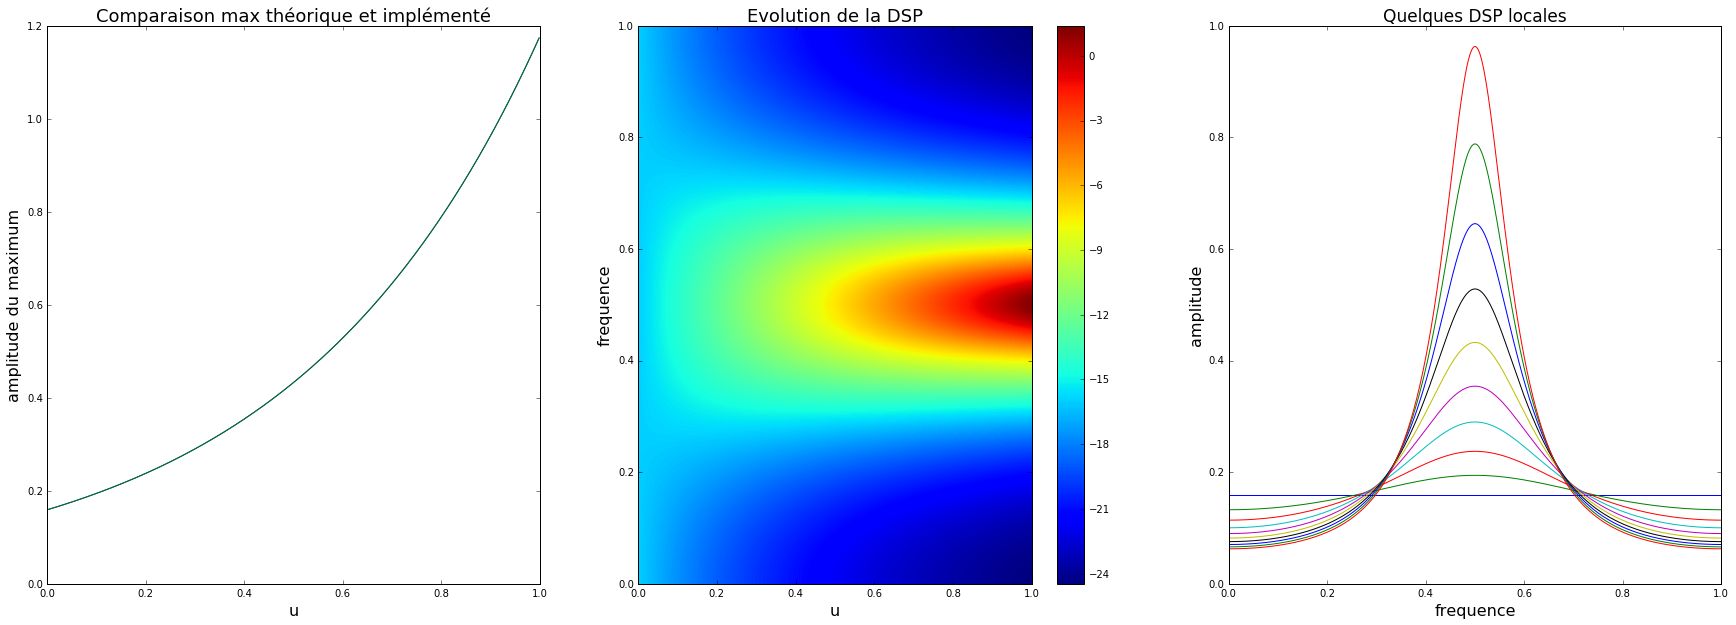
\includegraphics[scale=0.3]{presentation/images/TVAR1_module.png}
\caption{TVAR(1) avec $\phi$ fixe et $\rho$ variable. A gauche : $\rho(u)$ théorique et implémenté. Au milieu : évolution de la DSP. A droite : quelques DSP locales}
\label{fig:TVAR1_module}
\end{figure}

\begin{figure}[h]
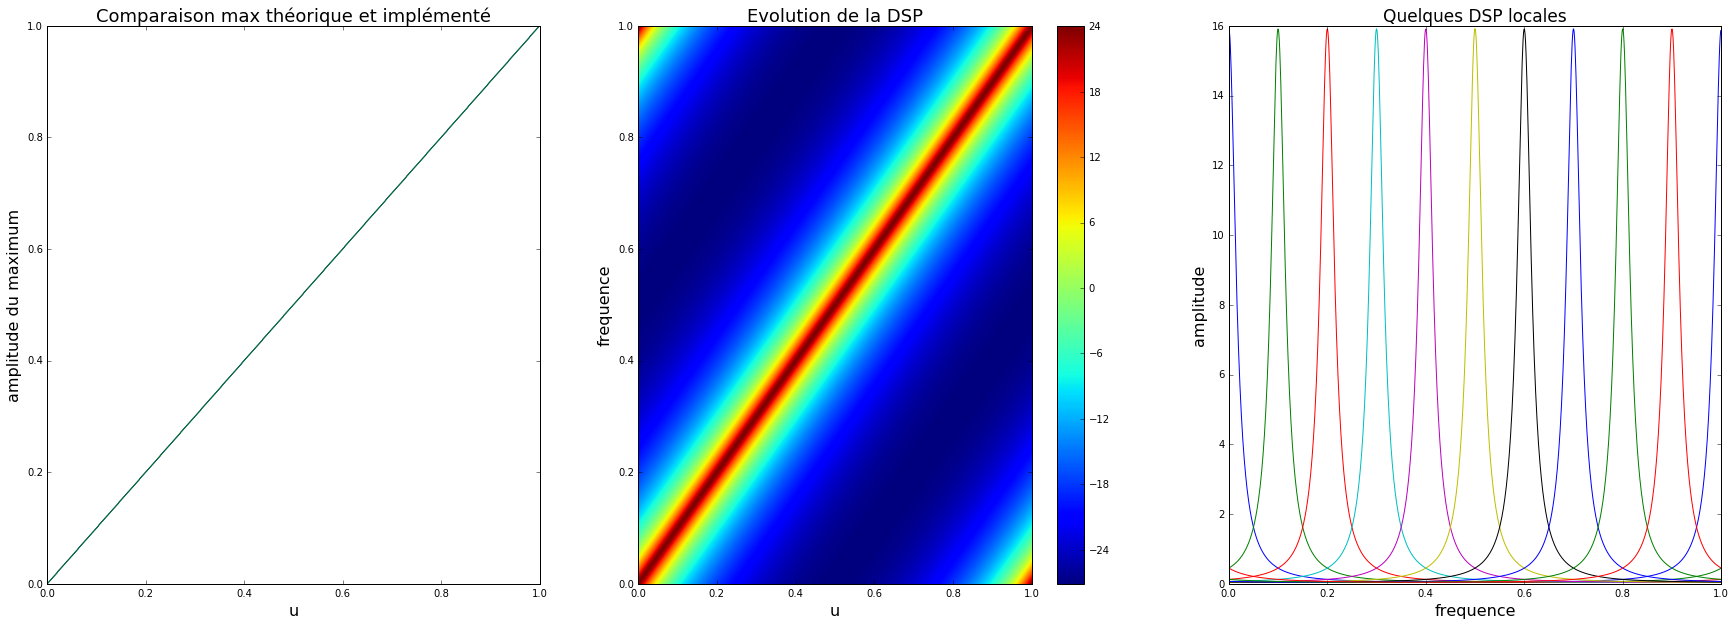
\includegraphics[scale=0.3]{presentation/images/TVAR1_phase.png}
\caption{TVAR(1) avec $\rho$ fixe et $\phi$ variable. A gauche : $\phi(u)$ théorique et implémenté. Au milieu : évolution de la DSP. A droite : quelques DSP locales}
\label{fig:TVAR1_phase}
\end{figure}

\subsection{Cas d'un TVAR(2)}
Le polynôme TVAR(2) s'écrit : $\forall u$ dans $[0,1], \Theta(z;u) = 1 - \theta_1(u) z - \theta_2(u) z^2$.
Si on note $z_1(u)$ et $z_2(u)$ les inverse des racines du polynôme, on a 
$\theta_1(u) = z_1(u) + z_2(u)$ et $\theta_2(u) = -z_1(u) z_2(u)$. La figure
\ref{fig:TVAR2_reelle} montre la trajectoire du processus pour différentes valeurs de $T$ et pour $z_1(u) = \frac{1}{2 + u}$ et $z_2(u) = \frac{1}{5 + \sin(2 \pi u)}$. Le processus généré est bien stable. 

La figure \ref{fig:TVAR2_conjuguees} montre les résultats obtenues pour $z_1(u) = \overline{z_2(u)}=\rho(u)e^{i\phi(u)}$ avec $\rho(u)=0.5$ et $\phi(u)=u/2$. Comme montré dans l'exemple \ref{ex:TVAR2}, on voit que le maximum de la DSP n'est pas vraiment au niveau de la phase. 

\begin{figure}[h]
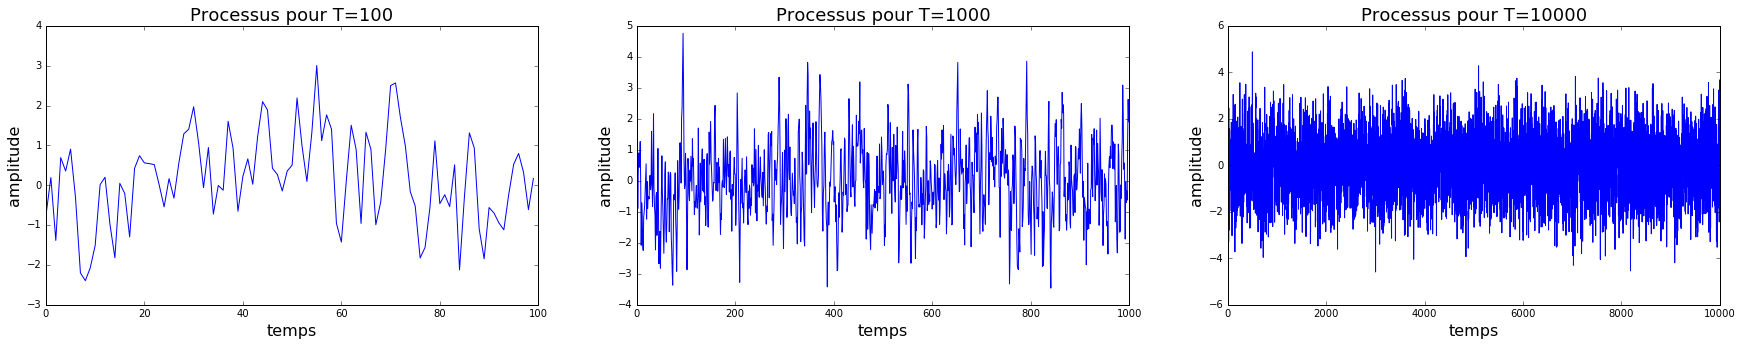
\includegraphics[scale=0.3]{presentation/images/TVAR2_racines_reelles.png}
\caption{TVAR(2) avec racines réelles}
\label{fig:TVAR2_reelle}
\end{figure}

\begin{figure}[h!]
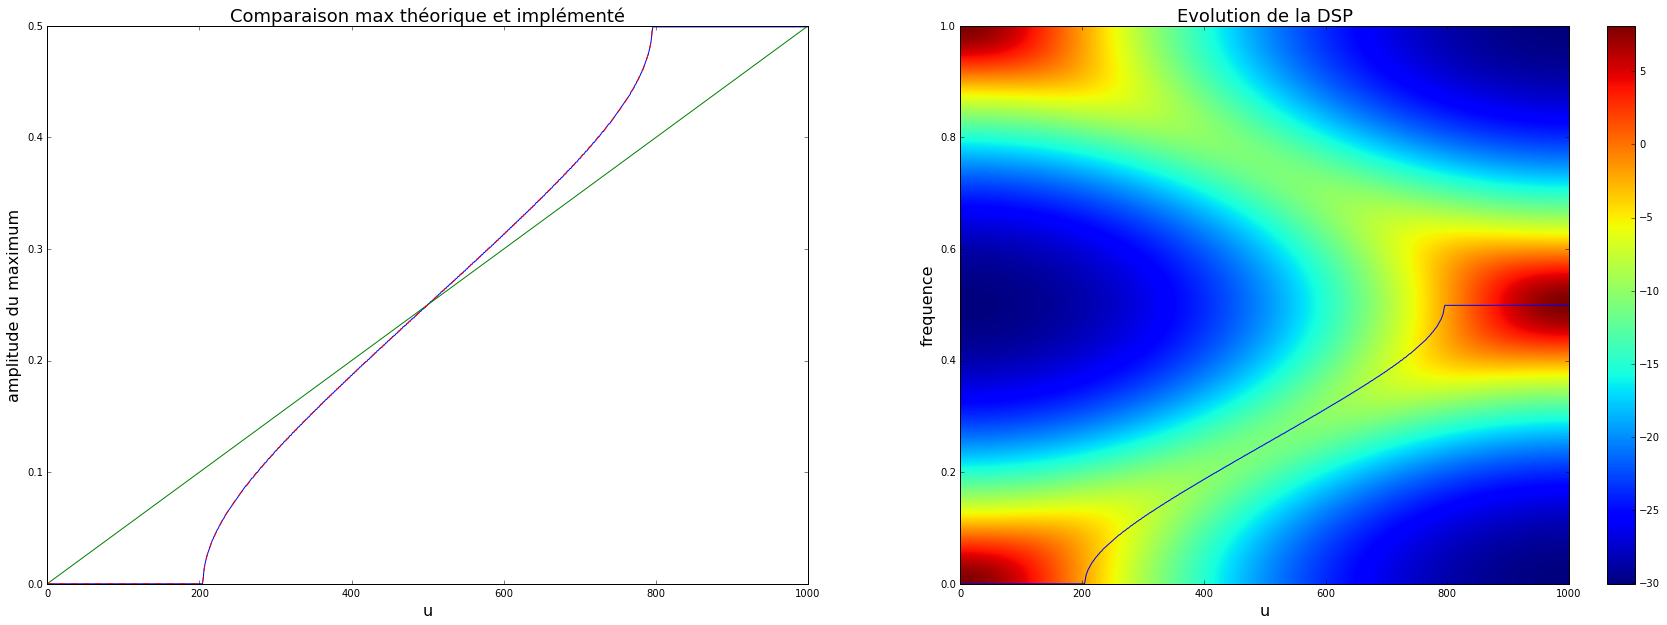
\includegraphics[scale=0.3]{presentation/images/TVAR2_racines_conjuguees.png}
\caption{TVAR(2) avec racines conjuguées. A gauche : $\phi(u)$ et max de la DSP. Au droite : évolution de la DSP.}
\label{fig:TVAR2_conjuguees}
\end{figure}
\pagebreak
\section{Génération et prédiction d'un TVAR(p)}
\subsection{Génération à partir des autocorrélations partielles}
On applique l'algorithme \ref{algo:construction} pour tout $t \in \iseg{1,T}$, les résultats sont présentés en figure \ref{fig:TVARd}. On remarque que le processus est bien stable.

\begin{figure}[h!]
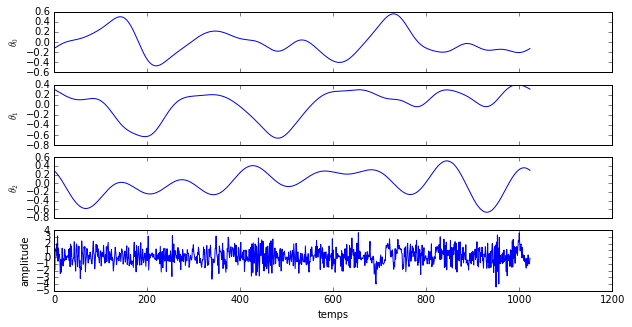
\includegraphics[scale=0.8]{presentation/images/TVARd.png}
\caption{TVAR(3) et les coefficients du polynôme. De haut en bas : $\theta_1, \theta_2, \theta_3$ et le processus.}
\label{fig:TVARd}
\end{figure}

\subsection{Estimation par NLSM}
On applique l'algorithme NLSM pour plusieurs valeurs de $\mu$. La figure \ref{fig:TVARd_estim} présente les trois coefficients d'un TVAR(3) ainsi que leurs estimations et le processus ainsi que sa prédiction. La valeur de $\mu$ est importante : on remarque que si il est trop petit, on a du mal à estimer les coefficients car on ne varie pas assez et si il est trop grand, on varie trop pour estimer les coefficients.
\begin{figure}[h]
\begin{subfigure}{\textwidth}
\centering
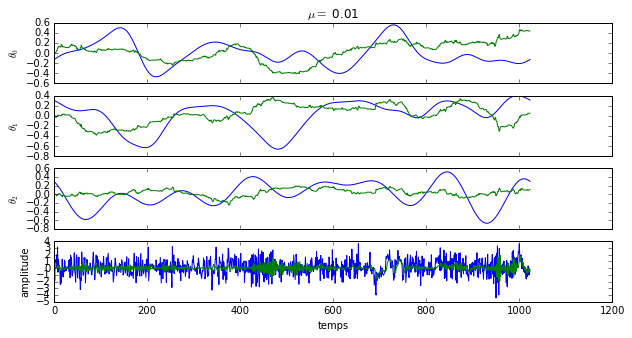
\includegraphics[scale=0.6]{presentation/images/TVARd_estim_mu001.png}
\caption{$mu = 0.01$}
\end{subfigure}
\begin{subfigure}{\textwidth}
\centering
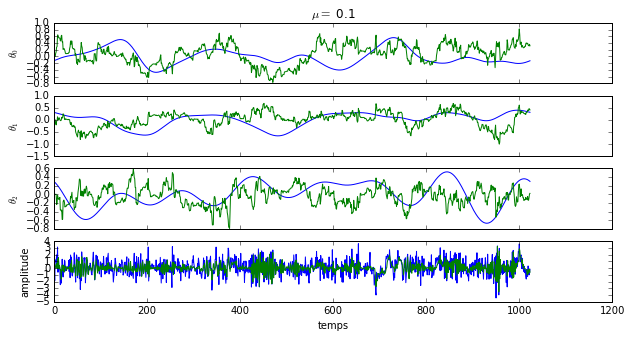
\includegraphics[scale=0.6]{presentation/images/TVARd_estim_mu01.png}
\caption{$mu = 0.1$}
\end{subfigure}
\begin{subfigure}{\textwidth}
\centering
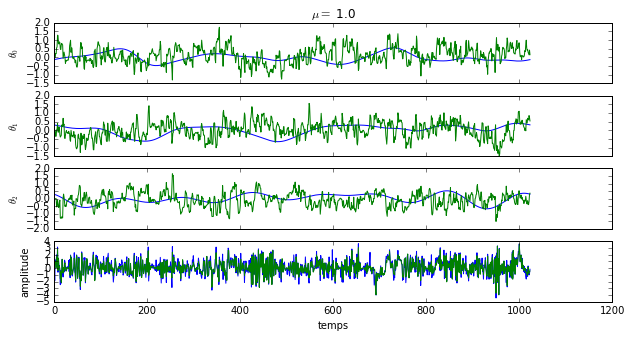
\includegraphics[scale=0.6]{presentation/images/TVARd_estim_mu1.png}
\caption{$mu = 1$}
\end{subfigure}
\caption{TVAR(3) et les coefficients du polynôme ainsi que les estimations et la prédiction. De haut en bas : $\theta_1, \theta_2, \theta_3$ et le processus.}
\label{fig:TVARd_estim}
\end{figure}

\section{Application à l'estimation d'un spectrogramme}
Dans cette section, on se propose d'estimer le spectrogramme d'un signal de parole. Le signal en entrée est la succession des voyelles "a-e-i-o-u". Il est connu que l'on peut modéliser les sons voisées grâce à des processus AR en supposant que le signal est localement stationnaire. Les processus TVAR tenant en compte l'évolution possible dans le temps des coefficients TVAR, nous avons pensé qu'il serait intéressant d'observer les résultats de l'estimateur TVAR sur un signal de parole. La figure \ref{fig:parole} montre que le résultat est assez convenable. Pour estimer le spectrogramme, on estime les coefficients TVAR puis on calcule les DSP locales à chaque instant.

\begin{figure}[h!]
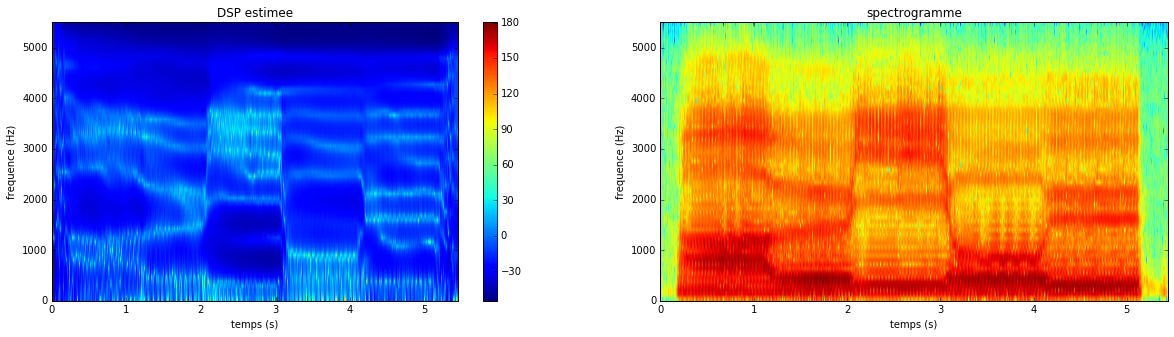
\includegraphics[scale=0.45]{presentation/images/parole.png}
\caption{Estimation du spectrogramme du signal "a-e-i-o-u". A gauche : sprectrogramme estimé. A droite : spectrogramme}
\label{fig:parole}
\end{figure}

\pagebreak
\phantomsection
\addcontentsline{toc}{chapter}{Bibliographie}
\bibliographystyle{plain}
\bibliography{biblio}
\end{document} 
